\documentclass[12pt,a4paper,twoside]{article}


% Encoding settings
\usepackage[utf8]{inputenc} % File encoding
\usepackage[T1]{fontenc}    % Font encoding
\usepackage{lmodern}        % Modern font

% Language settings
\usepackage[german]{babel} % Multi-language support %english

% Citation settings
\usepackage{csquotes}
\usepackage[backend=biber, style=authoryear, citestyle=authoryear-comp, natbib=true]{biblatex} % Setup for biblatex with biber.
\addbibresource{zitierungen.bib} % The filename of your bibliography file.

% Hyperlinks in the document
\usepackage[colorlinks, linkcolor=blue, citecolor=blue, urlcolor=blue]{hyperref} % Makes links clickable and colored.

% Page layout
\usepackage[tmargin=30mm, bmargin=30mm, lmargin=30mm, rmargin=30mm]{geometry}
%to get rid of htop:
% 

% Paragraph formatting
\setlength\parindent{0pt}  % Kein horizontaler Einzug am Anfang von Absätzen
\setlength\parskip{6pt plus 2pt minus 1pt}  % Vertikaler Abstand mit etwas Flexibilität

% Formatting for more subsections
\usepackage{titlesec}
\titleclass{\subsubsubsection}{straight}[\subsection]

\newcounter{subsubsubsection}[subsubsection]
\renewcommand\thesubsubsubsection{\thesubsubsection.\arabic{subsubsubsection}}
\renewcommand\theparagraph{\thesubsubsubsection.\arabic{paragraph}} % optional; useful if paragraphs are to be numbered

\titleformat{\subsubsubsection}
  {\normalfont\normalsize\bfseries}{\thesubsubsubsection}{1em}{}
\titlespacing*{\subsubsubsection}
{0pt}{3.25ex plus 1ex minus .2ex}{1.5ex plus .2ex}

\makeatletter
\renewcommand\paragraph{\@startsection{paragraph}{5}{\z@}%
  {3.25ex \@plus1ex \@minus.2ex}%
  {-1em}%
  {\normalfont\normalsize\bfseries}}
\renewcommand\subparagraph{\@startsection{subparagraph}{6}{\parindent}%
  {3.25ex \@plus1ex \@minus .2ex}%
  {-1em}%
  {\normalfont\normalsize\bfseries}}
\def\toclevel@subsubsubsection{4}
\def\toclevel@paragraph{5}
\def\toclevel@paragraph{6}
\def\l@subsubsubsection{\@dottedtocline{4}{7em}{4em}}
\def\l@paragraph{\@dottedtocline{5}{10em}{5em}}
\def\l@subparagraph{\@dottedtocline{6}{14em}{6em}}
\makeatother

\setcounter{secnumdepth}{4}
\setcounter{tocdepth}{4}

% Essential packages for mathematics
\usepackage{amsmath, amssymb}
\usepackage{array}

% Graphics support
\usepackage{graphicx}

% Enhanced lists
\usepackage{enumitem}
\setlist[enumerate]{topsep=0pt}
\setlist[itemize]{topsep=0pt}
\setlist[description]{font=\normalfont, topsep=0pt}
\usepackage{listings}
\usepackage[T1]{fontenc}

\usepackage{xcolor}

\colorlet{punct}{red!60!black}
\definecolor{background}{HTML}{EEEEEE}
\definecolor{delim}{RGB}{20,105,176}
\colorlet{numb}{magenta!60!black}

\lstdefinelanguage{json}{
    basicstyle=\normalfont\ttfamily,
    numbers=left,
    numberstyle=\scriptsize,
    stepnumber=1,
    numbersep=8pt,
    showstringspaces=false,
    breaklines=true,
    frame=lines,
    backgroundcolor=\color{background},
    literate=
     *{0}{{{\color{numb}0}}}{1}
      {1}{{{\color{numb}1}}}{1}
      {2}{{{\color{numb}2}}}{1}
      {3}{{{\color{numb}3}}}{1}
      {4}{{{\color{numb}4}}}{1}
      {5}{{{\color{numb}5}}}{1}
      {6}{{{\color{numb}6}}}{1}
      {7}{{{\color{numb}7}}}{1}
      {8}{{{\color{numb}8}}}{1}
      {9}{{{\color{numb}9}}}{1}
      {:}{{{\color{punct}{:}}}}{1}
      {,}{{{\color{punct}{,}}}}{1}
      {\{}{{{\color{delim}{\{}}}}{1}
      {\}}{{{\color{delim}{\}}}}}{1}
      {[}{{{\color{delim}{[}}}}{1}
      {]}{{{\color{delim}{]}}}}{1}
      {ß}{{{\ss}}}{1}
}


% PDF links and configuration
\usepackage{xcolor, hyperref}
\hypersetup{
  pdftitle={Hier den Titel der Arbeit},
  pdfauthor={Hier den Author der Arbeit},
  pdfsubject={Stichworte, weiteres Stichwort},
  colorlinks=true,
  linkcolor=blue!60!black,
  citecolor=blue!60!black,
  urlcolor=blue!60!black,
  filecolor=green!60!black,
  pdfborder={0 0 0},
  bookmarksopen=true,
  unicode=true,
}

\usepackage{float} % Include this line

% Custom commands
\newcommand\myworries[1]{\textcolor{red}{#1}}
\newcommand{\smallbold}[1]{\noindent\textbf{\small #1}}
\newcommand{\sectionbreak}{\clearpage}
\titleformat{\section}[block]
  {\normalfont\Large\bfseries}
  {\thesection}{1em}{}
\titlespacing*{\section}{0pt}{\baselineskip}{\baselineskip}


\begin{document}
\begin{titlepage}

  \vfill
  {\bfseries\Huge Verbesserung der Token-Klassifikation in technischen Zeichnungen durch den Einsatz
von Transformer-basierten Modellen\par}
  \vfill

  \textbf{Lukas Kouba} \\
  Abgabedatum: 18.07.2024

  \vfill

  Betreuer: Prof. Dr.-Ing. Maik Thiele

  \vfill

  Fakultät für Informatik/Mathematik \\
  Hochschule für Technik und Wirtschaft Dresden
\end{titlepage}

\newpage
\tableofcontents
\newpage

\myworries{Kommentare fuer morgen:
Viele Daten in semistrukturierten Dokumenten aus diesen konnen nur Bilder und worter extrahiert werden und nicht die struktur an sich, z.B. Tabellen, Graphen
Kann so nicht embedded werden,
Diese Daten zuerst als PDF hier kann haufig der Text herausgezogen werden weil hinterlegt, von maschienen wie autocad aber alles in bezierkurven gezeichnet, also muss alles als png verarbeitet werden,
schwierig text von bild zu unterscheiden,
da nicht embedded werden kann muss extra auf klassifizierung trainiert werden,}

\section{Einleitung}
\subsection{Motivation}
Für große Ingenieur- und Beratungsunternehmen mit einer Vielzahl von Dokumenten ist es ein erheblicher Aufwand, diese Dokumente den entsprechenden Projekten zuzuordnen und korrekt zu kennzeichnen. Die fortschreitende Digitalisierung bietet eine hervorragende Möglichkeit, die Kategorisierungsarbeit präziser und schneller zu gestalten. Methoden, die sowohl den Textinhalt als auch das Layout berücksichtigen, sind dabei von entscheidender Bedeutung, da sich Dokumente oft schon durch die Anordnung von Text, Bildern und deren jeweilige Größe unterscheiden. Donut und LayoutLM sind für solche Aufgaben besonders geeignet, da sie durch ihre Transformer-Architekturen sowohl den Textinhalt als auch das visuelle Layout von Dokumenten analysieren können.

\subsection{Ziele der Arbeit}
Das Hauptziel dieser Arbeit ist die Entwicklung einer Pipeline zur Extraktion von Metadaten aus umfangreichen technischen Zeichnungen.

Die Pipeline soll eine robuste, automatisierte Lösung darstellen, bei der die Dokumente von PDFs in Bilder transformiert werden und anschließend mit den in dieser Arbeit entwickelten Modellen Donut und LayoutLMv3, die auf der Transformationsarchitektur einer Deep Learning Methode basieren, verarbeitet werden, um bestimmte Metadaten zu extrahieren, auf deren Basis die Dokumente eindeutig kategorisiert werden können. Anschließend findet eine Nachbearbeitung statt, bei der versucht wird, nicht erfolgreich gefundene Metadaten zu bereinigen und dennoch zu extrahieren und gleichzeitig Metadaten mit sehr geringer Wahrscheinlichkeit der Richtigkeit auszusortieren, zu identifizieren und zur manuellen Bearbeitung weiterzuleiten. Die Genauigkeit und Praktikabilität der verwendeten Modelle wird evaluiert, um die Leistungsfähigkeit und Anwendbarkeit der Pipeline zu bestimmen.

\subsection{Dokumentverarbeitung}
Die Dokumentenverarbeitung spielt eine zentrale Rolle in der modernen Datenverarbeitung und umfasst die Erfassung, Analyse, Speicherung und Verwaltung von Informationen aus unterschiedlichen Dokumentenquellen. Dies ist besonders relevant für Organisationen, die große Mengen an Dokumenten verarbeiten müssen. Eine effiziente Dokumentenverarbeitung stellt sicher, dass Informationen schnell zugänglich, richtig kategorisiert und sicher archiviert werden.

Ein wesentlicher Aspekt der Digitalisierung ist die Umwandlung von physischen in digitale Dokumente, was die Speicherung vereinfacht und den Zugriff und die Verteilung von Informationen beschleunigt. Die Dokumentenlayoutanalyse ermöglicht es, die Struktur von Dokumenten zu erkennen und Textblöcke, Tabellen, Bilder und Überschriften zu identifizieren. Diese Elemente sind entscheidend für eine angemessene Kategorisierung und Indexierung, die die Suche und Nutzung von Informationen optimiert.

Semi-strukturierte Dokumente stellen eine Herausforderung dar, da aus ihnen oft nur Bilder und Wörter extrahiert werden können, nicht aber die Struktur selbst, wie z.B. Tabellen oder Grafiken. Aus solchen Dokumenten, die häufig im PDF-Format gespeichert sind, können Texte extrahiert werden, wenn sie hinterlegt sind. Bei technischen Zeichnungen, die häufig mit Software wie AutoCAD erstellt werden, sind die Elemente jedoch als Bezierkurven gezeichnet, was eine Verarbeitung im PNG-Format erforderlich macht. Die Schwierigkeit, Text von Bildern zu unterscheiden, und die Unmöglichkeit, sie direkt einzubetten, erfordern ein spezielles Training der Klassifizierungsalgorithmen, um eine effiziente Verarbeitung zu gewährleisten.

\subsection{Schlussfolgerung}
Die umfassende Verarbeitung und Analyse von Dokumenten ist entscheidend, um Arbeitsprozesse zu optimieren und das Informationsmanagement in Organisationen effektiver zu gestalten. Durch die gleichberechtigte Berücksichtigung von strukturierten und unstrukturierten Daten kann eine vollständige und durchsuchbare Dokumentenbasis geschaffen werden, die eine entscheidende Ressource für die Entscheidungsfindung und strategische Planung darstellt.
\section{Grundlagen und Theorien}
% \subsection{Überblick über verwandte Modelle}
% In der Dokumentenverarbeitung und Layouterkennung gibt es mehrere relevante Modelle und Technologien, die unterschiedliche Aspekte dieser Prozesse abdecken. Ein kurzer Überblick über einige dieser Modelle und Technologien bietet Einblicke in ihre Funktionsweise und Anwendungsbereiche.

% Optical Character Recognition (OCR) ist eine der grundlegendsten Technologien in der Dokumentenverarbeitung. OCR-Systeme verwenden Algorithmen zur Erkennung und Umwandlung von gedrucktem oder handgeschriebenem Text in maschinenlesbaren Text. Diese Technologie ist besonders nützlich für die Digitalisierung und Automatisierung der Texterfassung aus physischen Dokumenten.

% YOLO (You Only Look Once) ist ein neuronales Netzwerkmodell, das in erster Linie für die Objekterkennung in Bildern entwickelt wurde, aber auch für die Layouterkennung in Dokumenten angewendet werden kann. YOLO zeichnet sich durch seine Fähigkeit aus, Objekte in Echtzeit zu erkennen und ihre Positionen in Bildern zu bestimmen. In der Layouterkennung kann YOLO verwendet werden, um verschiedene Layoutkomponenten wie Textblöcke, Bilder und Tabellen in einem Dokument zu identifizieren und zu klassifizieren.

% Neben OCR und YOLO gibt es spezialisierte Modelle wie LayoutLM und Donut, die beide Transformer-Architekturen nutzen, um den Textinhalt und das Layout eines Dokuments gleichzeitig zu analysieren. LayoutLM integriert Layout- und Textinformationen in einem einzigen Modell und ist in der Lage, das relative Layout von Textblöcken zu verstehen und zu nutzen, um den Inhalt präzise zu klassifizieren. Donut hingegen fokussiert sich auf die Erkennung und Extraktion von Informationen aus Dokumenten, indem es sowohl strukturierten als auch unstrukturierten Text im Kontext seines Layouts interpretiert.
\subsection{Donut - Document Understanding Transformer}
Donut markiert einen entscheidenden Durchbruch in der Verarbeitung und Analyse von Dokumenten durch den Einsatz von Transformer-Technologien, ohne auf traditionelle OCR (Optical Character Recognition) Methoden angewiesen zu sein. Das Modell integriert fortschrittliche Verfahren wie den Swin Transformer, der die Analyse durch seine hierarchische Struktur und die effiziente Verarbeitung von Self-Attention erheblich beschleunigt. Donut ist in der Lage, Dokumente beliebiger Größe und Komplexität - einschließlich Text und eingebetteten Bildern - zu verarbeiten.

Der Swin Transformer optimiert die Verarbeitung, indem er die Daten in kleinere, überschaubare Patches aufteilt, die unabhängig voneinander verarbeitet werden können. Die Fähigkeit, nahtlos zwischen Text- und Bildelementen zu wechseln und diese im Kontext zu verstehen, ermöglicht Donut eine umfassende und tiefgreifende Analyse von Dokumenten. Diese Technologie ermöglicht nicht nur eine schnelle und effiziente Verarbeitung, sondern auch eine genaue und kontextbezogene Interpretation des Inhalts, was sie ideal für eine Vielzahl von Anwendungen in Bereichen macht, in denen eine schnelle und genaue Analyse von Dokumenten kritisch ist.
\myworries{Hier vielleicht noch eine Architekturubersicht wie bei LayoutLM einfugen welche SWIN Transformer als Encoder und Bert als Decoder darstellt?}
\subsubsection{Terminologie}

\smallbold{Transformer}\\
Transformer-Modelle sind eine Klasse von deep neural networks,die speziell für die Verarbeitung großer Mengen sequentieller Daten entwickelt wurden, wie sie typischerweise in der Sprachverarbeitung vorkommen. Ursprünglich in der Arbeit „Attention is all you need” \cite{Attention-Is-All-You-Need} vorgestellt, zeichnen sich diese Modelle durch einen Mechanismus namens Self-Attention aus, der es einem Modell ermöglicht, die Bedeutung eines Wortes im Kontext der anderen Wörter des Satzes zu gewichten.

\smallbold{Attention}\\
Das Attention-Prinzip im Kontext von Transformer-Modellen ermöglicht es, wichtige Informationen aus großen Datenmengen herauszufiltern und gleichzeitig weniger relevante Details zu minimieren. Dies ist besonders nützlich bei der Verarbeitung von Dokumenten, wo es darauf ankommt, schnell und effizient die entscheidenden Informationen zu extrahieren. 
In der Praxis funktioniert Attention durch die Berechnung von drei Hauptkomponenten: den Querys (Abfragen), Keys (Schlüsseln) und Values (Werten). Für jedes Element des Inputs erzeugt das Modell eine Query und vergleicht diese  mit allen Keys der anderen Elemente mittels eines Skalarprodukts. Das Ergebnis sind Scores, die angeben, wie relevant jedes andere Element des Inputs in Bezug auf das aktuelle Element ist.

\smallbold{Patches}\\
In der Anwendung von Transformer-Technologien, insbesondere in Modellen wie dem Swin Transformer, bezeichnet der Begriff „Patches” kleine, zusammenhängende Segmente eines Bildes oder Dokuments, die unabhängig voneinander analysiert und verarbeitet werden können. Patches ermöglichen eine effiziente Verarbeitung großer Datenmengen, indem sie die Komplexität der Daten reduzieren und den Aufmerksamkeitsmechanismus auf lokal relevante Informationen konzentrieren. Diese Segmentierung hilft, die Rechenlast zu verteilen und die Verarbeitung zu beschleunigen, indem die parallele Verarbeitung mehrerer Datenabschnitte gleichzeitig ermöglicht wird.




\subsubsection{Swin Transformer}

Die Vision Transformer (ViT) Technologie steht vor zwei wesentlichen Herausforderungen: Erstens, die konstante Patchgröße von 16x16 Pixeln ist oft nicht ausreichend für die Erkennung feiner Details. Zweitens führt der Attention-Mechanismus, bei dem jeder Patch mit jedem anderen kommuniziert, zu einer Laufzeitkomplexität von \(O(N^2)\), wobei \(N\) die Anzahl der Pixel bezeichnet. Der Swin Transformer adressiert beide Probleme effektiv.

\begin{figure}[H]
    \centering
    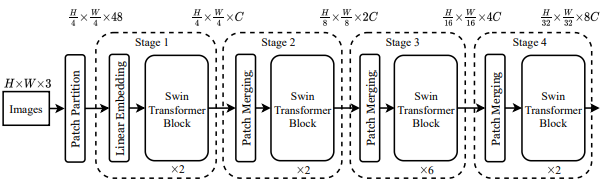
\includegraphics[width=0.7\linewidth]{SWIN-Transformer-Architektur.png}
    \caption{Architektur des Swin Transformers}
    \label{fig:swin_arch}
\end{figure}

Der Swin Transformer verwendet eine hierarchische Architektur, die aufeinanderfolgende Blöcke von W-MSA (Window Multi-head Self Attention) und SW-MSA (Shifted Window Multi-head Self Attention) beinhaltet.
\begin{figure}[H]
    \centering
    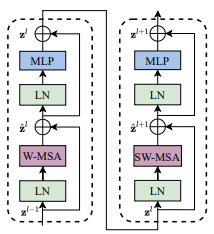
\includegraphics[width=0.2\linewidth]{SWIN-Transformer-Block.png}
    \caption{Zwei aufeinanderfolgende Swin-Transformerblöcke}
    \label{fig:enter-label}
\end{figure}

\textbf{W-MSA (Window Multi-head Self Attention)}\\
Der W-MSA-Ansatz unterteilt das Bild in nicht überlappende Fenster („Windows“), sodass jedes Fenster unabhängig durch den Multi-head Self Attention-Prozess verarbeitet wird. Dies reduziert die Laufzeitkomplexität von \(O(N^2)\) auf \(O(M \times N)\), wobei \(M\) die Anzahl der Fenster darstellt. Dieser Ansatz ist effektiv, da zwischen weit auseinander liegenden Pixeln wie denen in der linken oberen und der rechten unteren Ecke in der Regel kein relevanter Zusammenhang besteht.

\begin{figure}[H]
    \centering
    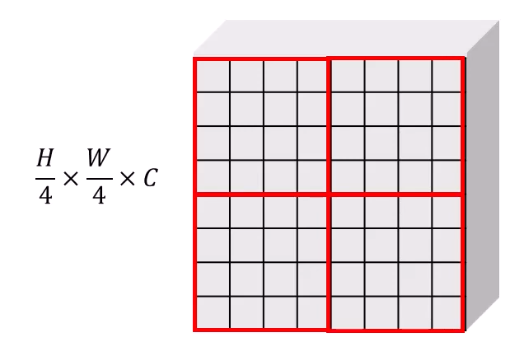
\includegraphics[width=0.25\linewidth]{SWIN-Transformer-WMSA.png}
    \caption{Zerlegung eines Bildes durch W-MSA}
    \label{fig:wmsa}
\end{figure}

Es treten jedoch zwei Probleme auf: Erstens, das Verschieben von Windows, um Attention über benachbarte Fenster hinweg zu ermöglichen, ist aufwendig. Dies würde dazu führen, dass anstelle von vier Fenstern neun benötigt werden, wobei zusätzlich Zero Padding angewendet werden muss, um die Bereiche außerhalb des Bildes abzudecken. Diese Berechnungen sind oft unnötig.

\begin{figure}[H]
    \centering
    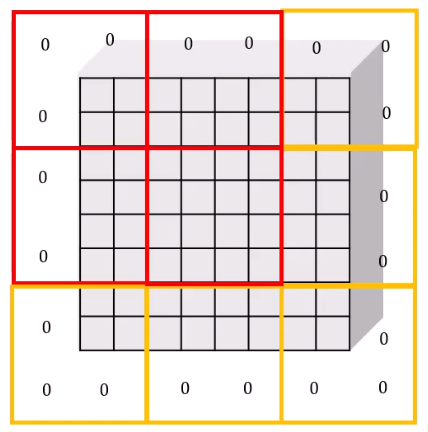
\includegraphics[width=0.3\linewidth]{SWIN-Transformer-Padding.png}
    \caption{Swin-Transformer Fensterverschiebung}
    \label{fig:window_shift}
\end{figure}

Zweitens, wenn ein Objekt erkannt wird, das sich über mehrere Fenster erstreckt. Der SW-MSA löst beide Probleme effizient.

\textbf{SW-MSA (Shifted Window Multi-head Self Attention)}\\
Im Gegensatz zur ursprünglichen Annahme, dass Fenster verschoben werden, findet beim SW-MSA tatsächlich eine Verschiebung der Patches selbst statt, durch einen Prozess, der als „Rolling“ bekannt ist. Dies eliminiert die Notwendigkeit für zusätzliche Fenster und Padding.

\begin{figure}[H]
    \centering
    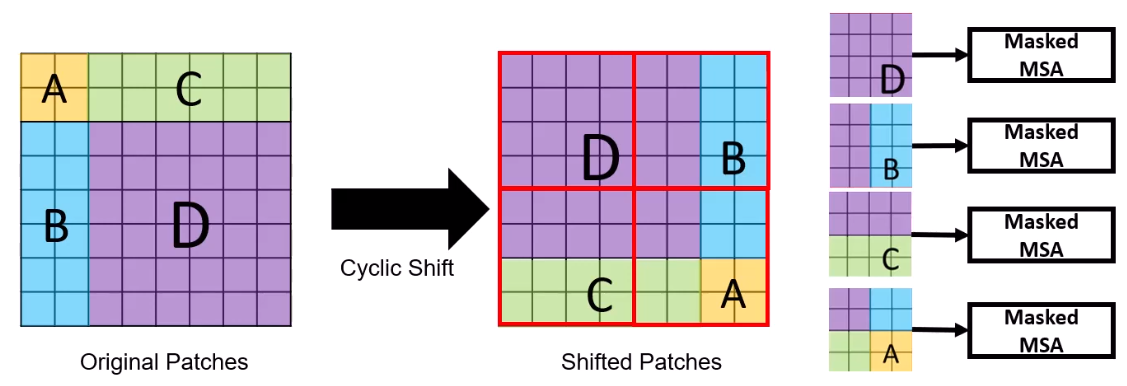
\includegraphics[width=0.7\linewidth]{SWIN-Transformer-SWMSA.png}
    \caption{Rolling und die daraus resultierenden neuen Fenster}
    \label{fig:swmsa}
\end{figure}

Masked MSA wird angewendet, da nach dem Rolling benachbarte Patches, die vorher weit voneinander entfernt waren, nebeneinander liegen und in der Regel keine relevante Attention benötigen. Diese werden daher „maskiert“, um unerwünschte Attention-Berechnungen zu verhindern.

\textbf{Patch Merging}\\\\
\smallbold{Definition von Kanälen}\\
In der digitalen Bildverarbeitung, besonders in modernen Netzwerkarchitekturen wie dem Swin Transformer, bezeichnet der Begriff \textit{Kanäle} (\(C\)) die Dimensionen der Daten, die spezifische Eigenschaften eines Bildes darstellen. In einem typischen RGB-Bild repräsentieren drei Kanäle die Farben Rot, Grün und Blau. In Transformer-basierten Architekturen, wie dem Swin Transformer, werden Kanäle genutzt, um die unterschiedlichen Merkmalsrepräsentationen der Daten zu verwalten.

\smallbold{Bedeutung und Erstellung von Feature Maps in Transformern}\\
In Transformer-Modellen werden Feature Maps nicht durch traditionelle Konvolutionsfilter, sondern durch den Mechanismus der Selbst-Attention generiert. Bei dieser Methode wird das Eingabebild in Patches zerlegt, die jeweils in höherdimensionale Vektoren transformiert werden. Diese Vektoren werden dann durch Multi-Head Attention verarbeitet, wobei jede "Head" unterschiedliche Aspekte der Daten betrachtet. Das Ergebnis dieser Prozesse sind kontextualisierte Feature Maps, die reiche und dynamische Repräsentationen jedes Patches darstellen. Diese Maps enthalten Informationen über die Beziehungen und Interaktionen zwischen verschiedenen Teilen des Bildes, was für komplexe Erkennungsaufgaben entscheidend ist.

\textbf{Patch Merging Prozess}\\
Im Patch Merging-Prozess des Swin Transformers werden vier benachbarte Patches zu einem größeren Patch zusammengefasst. Dieser Vorgang führt zu einer Vervierfachung der Kanalanzahl, da jedes ursprüngliche Patch seine individuellen Feature-Maps in den neuen, größeren Patch einbringt. Anschließend wird eine lineare Einbettung verwendet, um die erhöhte Anzahl von Kanälen zu reduzieren. Diese Reduktion optimiert die Effizienz des Netzwerks, indem sie die Datenmenge verarbeitbar hält, während sie gleichzeitig die wesentlichen Merkmale für die Erkennung von größeren Objekten in einem Fenster beibehält. Dies ermöglicht eine detailliertere Analyse der Merkmale in einem umfangreicheren Patch, was die Erkennung von umfangreichen Objekten verbessert.




\begin{figure}[H]
    \centering
    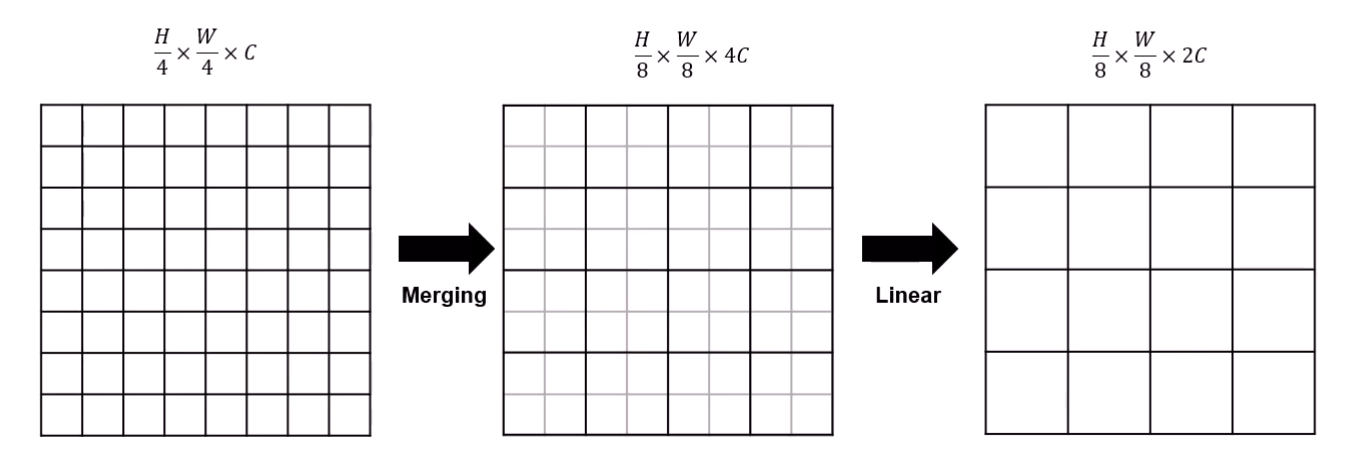
\includegraphics[width=0.7\linewidth]{SWIN-Transformer-PatchMerging.png}
    \caption{Patch Merging Prozess}
    \label{fig:patch_merging}
\end{figure}

Dieser Prozess wird, wie in Abbildung 1 gezeigt, wiederholt, um den Kontext über das gesamte Bild hinweg zu erfassen.\\
Für die Bildklassifikation wird der Output der letzten Schicht durch eine lineare Schicht geleitet, um eindeutige Ergebnisse zu erzielen. \\
Bei Objekterkennung oder Bildsegmentierung wird der Output jeder Schicht als Feature verwendet.

\textbf{Performance des Swin-Transformers}\\
In der untenstehenden Tabelle werden verschiedene Konfigurationen des Swin Transformers hinsichtlich Parameteranzahl, Rechenoperationen (FLOPs) und Durchsatz sowie deren Top-1-Genauigkeit auf ImageNet präsentiert. Der Swin-T (Tiny) verwendet eine Eingabebildgröße von \(224^2\) Pixeln und erreicht eine Top-1-Genauigkeit von 81.3\% mit nur 29 Millionen Parametern und 4.5G FLOPs. Dies zeigt eine effiziente Balance zwischen Genauigkeit und Rechenbedarf.

Für größere Modelle wie den Swin-S und Swin-B, die ebenfalls mit einer Bildgröße von \(224^2\) Pixeln arbeiten, verbessert sich die Genauigkeit auf bis zu 83.0\% bzw. 83.5\% bei einem erhöhten Rechenaufwand von 8.7G und 15.4G FLOPs. Interessanterweise zeigt der Swin-B, trainiert mit einer höheren Auflösung von \(384^2\) Pixeln, eine weitere Steigerung der Genauigkeit auf 84.5\%, was die Skalierbarkeit und Effektivität dieser Architektur unterstreicht.

Diese Ergebnisse verdeutlichen die hohe Leistungsfähigkeit des Swin Transformers, besonders im Vergleich zu anderen modernen Netzwerkarchitekturen wie den verschiedenen RegNet- und Vision Transformer-Modellen. Der Swin Transformer stellt somit eine vielversprechende Wahl für anspruchsvolle Aufgaben in der Bilderkennung dar.
\begin{figure}[H]
    \centering
    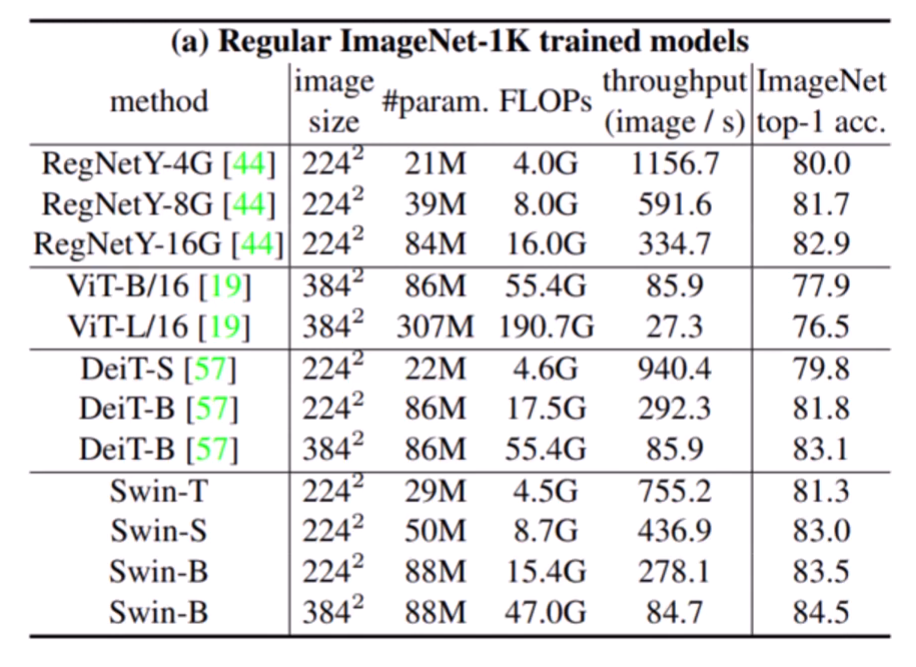
\includegraphics[width=0.6\linewidth]{SWIN-Transformer-Performance.png}
    \caption{Vergleich des Swin-Transformers mit anderen Modellen}
    \label{fig:enter-label}
\end{figure}

\cite{SWIN-Transformer-Paper}
\cite{SWIN-youtube}



\subsubsection{BART: Bidirectional and Auto-Regressive Transformers}

BART vereint die Stärken von zwei revolutionären Ansätzen in der Verarbeitung natürlicher Sprache: BERT (Bidirectional Encoder Representations from Transformers) und GPT (Generative Pre-trained Transformer). Diese Synthese ermöglicht es BART, sowohl textverstehende als auch textgenerierende Aufgaben effektiv zu bewältigen. Hierbei kombiniert BART die bidirektionale Kodierungsfähigkeit von BERT mit der autoregressiven Textgenerierungskapazität von GPT, was es zu einem flexiblen Werkzeug für eine Vielzahl von NLP-Aufgaben macht.

\textbf{Architektur}\\
BART ist als Sequence-to-Sequence-Modell konzipiert, das einen Encoder für die Analyse des Eingabetextes und einen Decoder zur Texterzeugung umfasst.\\
Der bidirektionale Encoder verarbeitet den Eingabetext in beide Richtungen, was bedeutet, dass Kontextinformationen sowohl von links nach rechts als auch von rechts nach links integriert werden. Dies ermöglicht ein tiefes Verständnis der semantischen Zusammenhänge innerhalb des Textes.

\begin{figure}[H]
    \centering
    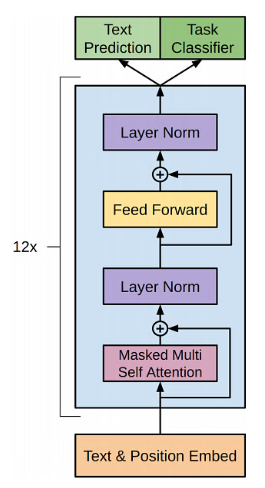
\includegraphics[width=0.2\linewidth]{BART-Decoder.png}
    \caption{Decoder Architektur von BART}
    \label{fig:enter-label}
\end{figure}

Der autoregressive Decoder erzeugt den Ausgabetext, indem er jedes folgende Token auf der Grundlage aller zuvor erzeugten Token vorhersagt. Dieser Prozess ist sequentiell und berücksichtigt den zuvor erzeugten Kontext, um kohärente Texte zu erzeugen. Die Architektur ist sehr ähnlich zu den Decodern der Vanilla-Transformer.


\textbf{Training durch Korruption und Rekonstruktion}

BART wird durch ein spezielles Verfahren trainiert, das auf der Korruption und anschließenden Rekonstruktion des Originaltextes basiert. Dieses Verfahren beinhaltet mehrere Strategien:

\begin{itemize}
    \item \textbf{Token Maskierung:} Zufällige Wörter oder Token werden durch ein spezielles Maskensymbol ersetzt, und das Modell lernt, diese zu rekonstruieren.
    \item \textbf{Satzpermutation:} Die Reihenfolge der Sätze wird zufällig verändert, und das Modell muss die ursprüngliche Ordnung wiederherstellen.
    \item \textbf{Dokumentrotation:} Der Text wird an einer zufälligen Stelle 'rotiert', sodass das Ende an den Anfang verschoben wird. Das Modell lernt, den Text in die korrekte Reihenfolge zu bringen.
    \item \textbf{Token Löschung:} Zufällige Token werden entfernt, und das Modell muss diese Lücken füllen.
    \item \textbf{Text Infilling:} Größere Textabschnitte werden durch Masken ersetzt, und das Modell füllt die fehlenden Inhalte. Es kann auch eine Maske eingesetzt werden, ohne einen Teil des Textes zu entfernen.
\end{itemize}

\textbf{Modellvergleich von BERT, GPT und BART}\\

\begin{figure}[H]
    \centering
    % Adjust the minipage widths to allocate space for each figure as needed
    \begin{minipage}[b]{0.2\linewidth}
        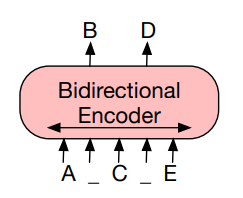
\includegraphics[width=\linewidth]{BART-Bert-erkleart.png}
        \caption{BERT}
        \label{fig:bert}
    \end{minipage}
    \hfill % Use \hfill to add horizontal space between the figures
    \begin{minipage}[b]{0.3\linewidth}
        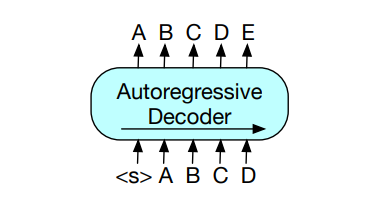
\includegraphics[width=\linewidth]{BART-Gpt-erklaert.png}
        \caption{GPT}
        \label{fig:gpt}
    \end{minipage}
    \hfill % Use \hfill to ensure the figures spread across the available space
    \begin{minipage}[b]{0.4\linewidth}
        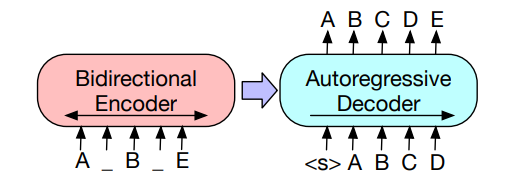
\includegraphics[width=\linewidth]{BART-Bart-erklaert.png}
        \caption{BART}
        \label{fig:bart}
    \end{minipage}
\end{figure}

\begin{itemize}
    \item[(Abbildung 9)] \textbf{BERT (Bidirectional Encoder Representations from Transformers):} Bei BERT werden zufällige Token durch Maskierungssymbole ersetzt und das Dokument bidirektional kodiert. Die fehlenden Token werden unabhängig voneinander vorhergesagt, was bedeutet, dass BERT nicht ohne Weiteres für die Textgenerierung eingesetzt werden kann.

    \item[(Abbildung 10)] \textbf{GPT (Generative Pre-trained Transformer):} Bei GPT werden Token autoregressiv vorhergesagt, was bedeutet, dass jedes Token basierend auf den bisher generierten Token vorhergesagt wird, was eine Nutzung für Textgenerierung ermöglicht. Allerdings kann GPT nur auf den linksseitigen Kontext konditionieren und lernt keine bidirektionalen Zusammenhänge.

    \item[(Abbildung 11)] \textbf{BART (Bidirectional and Auto-Regressive Transformers):} Bei BART müssen die Eingaben für den Encoder nicht mit den Ausgaben des Decoders übereinstimmen, was eine größere Flexibilität bei der Textkorruptionen ermöglicht. Das korrupte Dokument wird zuerst bidirektional kodiert und dann wird die Wahrscheinlichkeit des Originaldokumentes(rechts) durch einen autoregressiven Decoder berechnet. Für das Feintuning wird ein unverfälschtes Dokument sowohl in den Encoder als auch in den Decoder eingegeben, wobei die Repräsentationen aus dem finalen verborgenen Zustand des Decoders verwendet werden.
\end{itemize}

\textbf{Anwendungsbereiche}\\

Dank seiner vielseitigen Architektur und seines umfassenden Trainingsansatzes eignet sich BART für diverse NLP-Aufgaben:

\begin{itemize}
    \item \textbf{Textzusammenfassung:} Das Modell erstellt prägnante Zusammenfassungen längerer Texte.
    \item \textbf{Fragebeantwortung:} BART kann spezifische Informationen aus einem gegebenen Text extrahieren, um Fragen präzise zu beantworten.
    \item \textbf{Textgenerierung:} Es erzeugt textuelle Inhalte, die auf einer vorgegebenen Eingabe basieren.
    \item \textbf{Maschinenübersetzung:} Das Modell übersetzt Texte zwischen verschiedenen Sprachen.
    \item \textbf{Textklassifikation:} BART kann Texte bestimmten Kategorien zuordnen.
\end{itemize}

\textbf{Performance von BART}\\
\begin{figure}[H]
    \centering
    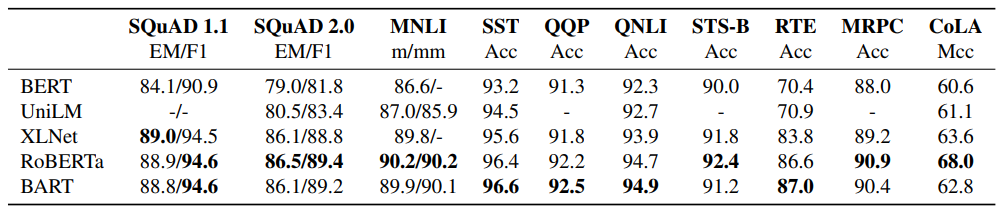
\includegraphics[width=0.6\linewidth]{BART-performance.png}
    \caption{BART im Vergleich zu anderen Modellen}
    \label{fig:1}
\end{figure}

Die Tabelle zeigt die Ergebnisse großer Modelle bei den SQuAD- und GLUE-Tests. BART wird hier im Vergleich zu anderen Modellen wie BERT, UniLM, XLNet und RoBERTa dargestellt. 

Im SQuAD 1.1 Benchmark erzielt BART eine EM/F1-Score von 88.8/94.6, was im Vergleich zu anderen Modellen, einschließlich XLNet und RoBERTa, wettbewerbsfähig ist. Bei SQuAD 2.0 erreicht BART eine EM/F1-Score von 86.1/89.2, wobei es ebenfalls ähnliche Ergebnisse wie RoBERTa erzielt, jedoch etwas hinter XLNet zurückbleibt.

In den GLUE-Tests zeigt BART bemerkenswerte Leistungen, insbesondere bei SST (96.6), QQP (92.5), QNLI (94.9) und STS-B (91.2). Diese Ergebnisse sind vergleichbar mit denen von RoBERTa und übertreffen in vielen Fällen die anderen Modelle. Besonders hervorzuheben ist die Leistung von BART bei den MNLI-Tests (89.9/90.1), wo es die höchste Punktzahl erreicht.

Die Ergebnisse verdeutlichen, dass die uni-direktionalen Decoder-Schichten von BART die Leistung bei diskriminativen Aufgaben nicht mindern. Vielmehr zeigt BART eine starke Performance, die mit den besten derzeit verfügbaren Modellen konkurriert.


\subsubsection{Donut Encoder-Decoder Modell}

\begin{figure}[H]
\centering
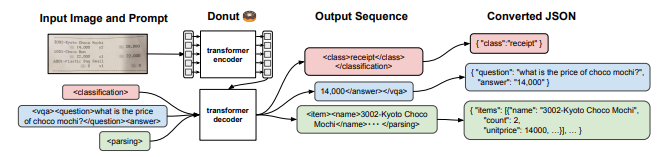
\includegraphics[width=0.6\linewidth]{DONUT-Input-Output.png}
\caption{Die Pipeline von Donut}
\label{fig:2}
\end{figure}

\textbf{Das Donut-Modell im Überblick}\\
Das Donut-Modell ist eine innovative Entwicklung im Bereich der Verarbeitung visueller Dokumente, die auf fortschrittlichen Transformer-Architekturen basiert. Kernstück ist der Swin Transformer, der für die Kodierung der visuellen Inhalte verantwortlich ist. Die Konfiguration des Swin Transformers in Donut besteht aus Schichten der Größe 2, 2, 14, 2 und einer Fenstergröße von 10. Diese Konfiguration stellt einen Kompromiss zwischen Geschwindigkeit und Genauigkeit dar und ermöglicht es dem Modell, Bilder mit einer maximalen Auflösung von 2560x1920 effizient zu verarbeiten. Diese Informationen werden an den Decoder weitergeleitet, der auf dem BART-Modell basiert.

\textbf{Konfiguration des BART Decoders}\\
Der BART-Decoder im Donut besteht aus vier Schichten und ist speziell dafür ausgelegt, die vom Encoder kommenden Informationen in Text umzuwandeln. Der Decoder verwendet eine maximale Tokensequenzlänge von 1536, wobei jedes Token durch einen One-Hot-Vektor mit der Größe des Vokabulars repräsentiert wird. Der Initialisierungsprozess des Decoders verwendet die Gewichte des zuvor trainierten multilingualen BART-Modells, was die Generalisierbarkeit und Effektivität des Donut-Modells bei der Verarbeitung von Dokumenten aus unterschiedlichen Sprachen und Kontexten erheblich verbessert.

\textbf{Eingabeprozedur und Aufgabenstellung}\\
Die Eingabeprozedur für das Modell verwendet das Teacher Forcing Schema, wobei Ground Truth als Eingabe verwendet wird, um das Training zu optimieren. Für jede spezifische Aufgabe werden den Prompts spezielle Tokens hinzugefügt, die die Art der Aufgabe definieren. Diese Prompts und ihre erwarteten Ausgaben sind in Abbildung 11 dargestellt und veranschaulichen die vielfältigen Anwendungsmöglichkeiten von Donut.

\textbf{Ausgabeformat und Strukturierung}\\
Die Ausgabe des Modells wird in ein strukturiertes JSON-Format konvertiert, das für die weitere Verarbeitung und Analyse geeignet ist. Diese Ausgabe enthält spezielle Token [START *] und [END *], die den Anfang und das Ende jedes zu extrahierenden Feldes kennzeichnen, wobei das Sternchen den Feldnamen darstellt.

\textbf{Pre-Training und Trainingsziele}\\
Das Pre-Training von Donut konzentriert sich auf die Erkennung von Texten in ihrer natürlichen Lesereihenfolge von links oben nach rechts unten und zielt darauf ab, den Cross-Entropy-Loss bei der Vorhersage des nächsten Tokens zu minimieren. Diese Trainingsmethode ermöglicht es Donut, die Genauigkeit der Token-Vorhersage auf der Basis des visuellen Kontextes und des vorherigen Textkontextes zu maximieren.

\cite{Donut-Paper}
\subsection{LayoutLMv3}

\begin{figure}[H]
    \centering
    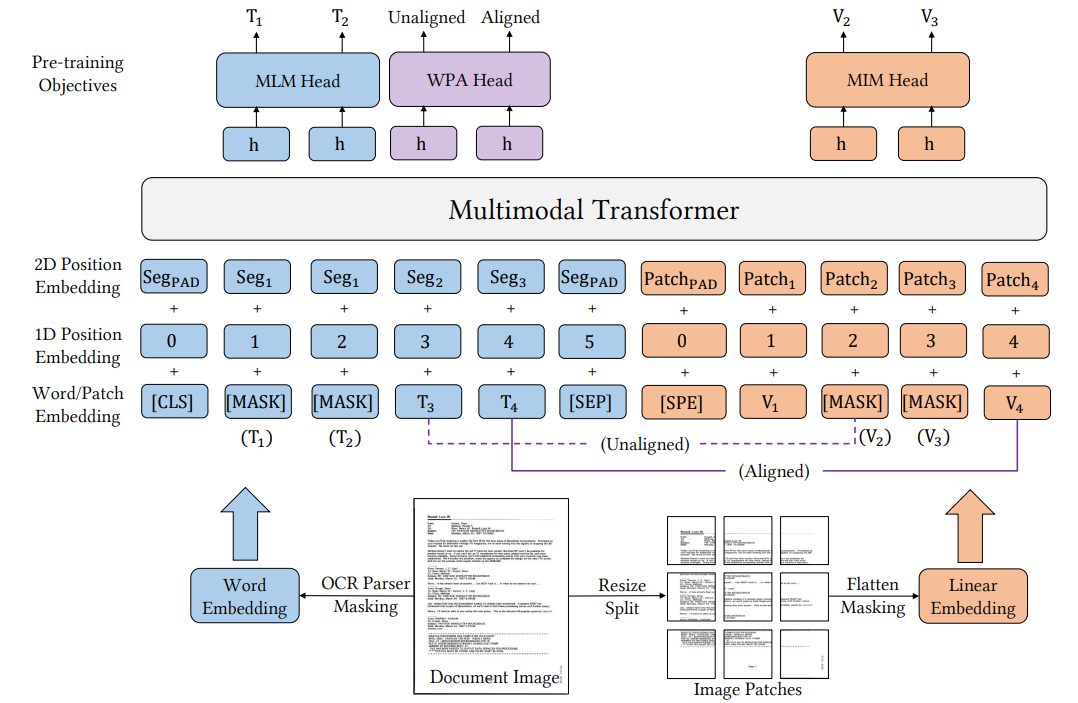
\includegraphics[width=0.8\linewidth]{LAYOUTLMV3-Architektur-Ueberblick.png}
    \caption{Überblick über die Architektur von LayoutLMv3}
    \label{fig:layoutlmv3-arch}
\end{figure}

LayoutLMv3 ist ein multimodales Transformer-Modell, das speziell dafür entwickelt wurde, Text- und Bild-Embeddings effizient zu kombinieren. Das Modell nutzt eine Architektur, die aus mehreren Schichten von Multi-Head Self-Attention und positionsspezifischen Feedforward-Netzwerken (FFN) besteht. Die Kerninnovation von LayoutLMv3 besteht darin, dass es Text- und Bildinformationen in einem einzigen Modell integriert, ohne dass eine vorherige Identifizierung der Bildelemente durch konventionelle Convolutional Neural Networks (CNNs) notwendig ist.


\subsubsection{Multimodaler Transformer für visuelle und textuelle Daten}

\textbf{Architektur-Übersicht}\\
Der multimodale Transformer LayoutLMv3 verwendet eine Dual-Stream-Architektur, die visuelle und textuelle Eingaben getrennt, aber parallel verarbeitet. Die Hauptkomponenten bestehen aus zwei getrennten Transformern, einem für Sprache und einem für visuelle Eingabe, sowie Co-Attention Transformer Layers, die die Integration und den Abgleich von Informationen aus der visuellen und der textuellen Domäne ermöglichen

\textbf{Eingabedarstellung}\\
Die textuelle Eingabe wird ähnlich wie bei BERT mit Hilfe von WordPiece-Embeddings tokenisiert, wobei spezielle Token wie \texttt{[CLS]} (für Klassifikationsaufgaben) und \texttt{[SEP]} (zur Trennung von Sätzen oder Segmenten) verwendet werden. Im Gegensatz zu LayoutLMv2, das Bilder mit einem vortrainierten CNN verarbeitet, verwendet LayoutLMv3 Techniken wie Masked Image Modeling (MIM), Masked Language Modeling (MLM) und Word Patch Alignment (WPA), um Korrespondenzen zwischen Text und Bildern herzustellen.
Dadurch wird es möglich, Begriffe wie „Apfel" direkt mit dem Bild eines Apfels im Embedding-Raum zu verknüpfen.

\textbf{Verarbeitungsströme}
Der Sprachfluss verarbeitet die Texteingabe durch mehrere Schichten von Transformer-Blöcken, die Multi-Head Self-Attention und vollständig verbundene Schichten verwenden und kontextabhängige Embeddings für jedes Worttoken erzeugen. \\
Der visuelle Stream verarbeitet Bild-Embeddings durch eine eigene Reihe von Transformer-Blöcken und erzeugt kontextabhängige Embeddings für jede Bildregion.

\textbf{Co-Attention-Mechanismus}\\
Eine der Schlüsselinnovationen multimodaler Transformer sind die Co-Attention Transformer-Schichten. In diesem Mechanismus arbeiten spezielle Co-Attention-Schichten abwechselnd mit den Standard-Self-Attention-Schichten, so dass die beiden unabhängigen Datenströme - Text und Bild - sich gegenseitig und ihre Embeddings beeinflussen können.
Innerhalb jeder Co-Attention-Schicht gibt es drei wesentliche Sublayer: 

Der \textbf{Self-Attention-Sublayer} erlaubt es jedem Datenstrom, seine Darstellung unabhängig zu verfeinern.
    
Die \textbf{Guided-Attention-Sub-layer} steuert den Aufmerksamkeitsmechanismus eines Datenstroms, um die Aufmerksamkeit auf relevante Teile des anderen Datenstroms zu lenken. Dies geschieht durch die Verwendung von Attention-Weights, die die Verteilung der Aufmerksamkeit im jeweils anderen Datenstrom beeinflussen. Auf diese Weise werden beispielsweise visuelle Informationen genutzt, um wichtige Textinformationen hervorzuheben und umgekehrt. Dadurch kann das Modell besser verstehen, welche Teile des Textes und des Bildes miteinander in Beziehung stehen und gemeinsam betrachtet werden sollten.

Die dritte Komponente, die \textbf{Feed-Forward-Sub-layers}, folgt auf jede Attention-Einheit. Die Feed-Forward-Sub-layers werden nach den Attention-Einheiten eingesetzt, um die durch die von den Attention-Einheiten erhaltenen Informationen weiter zu verarbeiten und zu verfeinern. Jede Feed-Forward-Sub-layer besteht aus zwei vollständig verbundenen Schichten mit einer nichtlinearen Aktivierungsfunktion dazwischen. Dies hilft dabei, komplexe Muster in den Daten zu erkennen und zu lernen. Der Zweck dieser Schichten besteht darin, die von den Aufmerksamkeitsmechanismen erzeugten Repräsentationen weiter zu verarbeiten, um tiefere und abstraktere Merkmale zu extrahieren. Durch die Abfolge von Attention- und Feed-Forward-Schichten kann das Modell sowohl kontextuelle Beziehungen als auch detaillierte Merkmale aus den Eingabedaten effektiv erfassen und nutzen.
    

\textbf{Trainingsziele}\\
In der ersten Phase des Trainings werden Bild- und Texttransformer separat trainiert, um zu kontrollieren, welchen Output der Transformer erzeugen soll. Zu Beginn wird der Text mit RoBERTa Word Embeddings initialisiert, um dem Transformer zu ermöglichen, diese während des Trainings zu optimieren. 
Der Bildstrom wird mit dem DiT(Document Image Transformer)-Vokabular initialisiert, um Label für Dokumente zu erzeugen, ursprünglich trainiert auf dem IIT-CDIP Datensatz.
    
In der zweiten Phase werden Bild- und Texteingaben gemeinsam trainiert, z.B. durch Masking-Techniken, um die Korrespondenz zwischen Bild und Text zu erlernen.
    
In der dritten Phase erfolgt die Feinabstimmung für spezifische Aufgaben wie Document Visual Question Answering (DocVQA), Klassifikation und andere Downstream-Tasks.


\subsubsection{Text-Embeddings}
Die Text-Embeddings in LayoutLMv3 werden durch eine Kombination aus Word-Embeddings und Position-Embeddings generiert. Diese Embeddings werden während des Preprocessings mittels Optical Character Recognition (OCR) erfasst. Die Word-Embeddings werden initial mit den Embeddings von RoBERTa initialisiert, einer der führenden Technologien in der Sprachverarbeitung. Die Position-Embeddings setzen sich zusammen aus 1D-Positionen, die die Position innerhalb der Token-Sequenz angeben und  2D-Positionen, die die Position der Tokens im Gesamtdokumentlayout beschreiben.

\subsubsection{Normierung und Positionsinformationen}
Ein entscheidender Aspekt von LayoutLMv3 ist die Normierung der Koordinaten jedes Wortes oder Segments in Relation zur Größe des Bildes oder Dokuments. Dies ermöglicht eine präzise und kontextbezogene Interpretation der Dokumentinhalte. Im Gegensatz zu früheren Versionen des Modells, die Positionsinformationen auf Wortebene verwenden, implementiert LayoutLMv3 segmentweise Positionsinformationen. Das bedeutet, dass alle Wörter innerhalb desselben Segments dieselben 2D-Positionsinformationen teilen, was zur besseren Erfassung semantischer Zusammenhänge beiträgt.

\subsubsection{Transformer-Input und Bildverarbeitung}
Der Input für den Transformer besteht aus einer Konkatenation der Text-Embeddings \(Y\) und Bild-Embeddings \(X\).
\begin{itemize}
    \item Die Bildrepräsentation \(I\) wird zuerst zu \(I \in \mathbb{R}^{C \times H \times W}\) verarbeitet.
    \item Anschließend wird das Bild in eine Sequenz von \(P \times P\) Patches unterteilt.
    \item Diese Patches werden linear auf eine Dimension \(D\) projiziert und zu einer Sequenz von Vektoren abgeflacht, deren Länge \(M = \frac{HW}{P^2}\) ist.
    \item Zu jedem dieser Patches werden lernbare 1D-Position-Embeddings hinzugefügt.
\end{itemize}

\subsubsection{Integration der Repräsentationstechniken}
LayoutLMv3 verwendet drei Haupttechniken zur Integration und Verarbeitung der multimodalen Daten: Masked Image Modeling (MIM), Masked Language Modeling (MLM) und Word Patch Alignment (WPA). Diese werden in einer gemeinsammen Loss-Funktion miteinander vereint: \[L = L_{\text{MLM}} + L_{\text{MIM}} + L_{\text{WPA}}\] Diese Techniken ermöglichen es dem Modell, sowohl textuelle als auch bildliche Inhalte effektiv zu interpretieren und die Beziehungen zwischen Text und Bild auf einer tieferen Ebene zu verstehen.

\textbf{Masked Language Modeling (MLM)}\\
30\% der Text-Tokens werden maskiert, wobei die Länge der maskierten Spannen aus einer Poisson-Verteilung mit einem Lambda von 3 gezogen wird. Das Ziel des Pretrainings ist es, die log-Likelihood der maskierten Text-Tokens \(y_l\) auf Basis des verfälschten Dokuments zu maximieren, wobei \(X^{M'}\) und \(Y^{L'}\) die maskierten Bild- und Text-Tokens bezeichnen. Die Loss-Funktion \(L_{MLM}(\theta)\) wird definiert als:
\[
L_{MLM}(\theta) = -\sum_{l=1}^{L'} \log p_{\theta}(y_l \mid X^{M'}, Y^{L'})
\]
Dies fördert das Erlernen der Korrespondenz zwischen Layout-Informationen sowie Text- und Bildkontext.

\textbf{Masked Image Modeling (MIM)}\\
Hier werden 40\% der Bild-Token mit einer blockweisen Maskierungsstrategie maskiert. Die Cross-Entropy wird verwendet, um den Inhalt der maskierten Bild-Tokens \(x_m\) zu rekonstruieren, wobei der umgebende Text und die Bildtokens als Kontext dienen:
\[
L_{MIM}(\theta) = -\sum_{m=1}^{M'} \log p_{\theta}(x_m \mid X^{M'}, Y^{L'})
\]

\textbf{Word Patch Alignment (WPA)}\\
Das Hauptziel des Word Patch Alignment (WPA) besteht darin, eine präzise Abstimmung zwischen Textwörtern und den entsprechenden Bildfeldern herzustellen. Eine Herausforderung bei herkömmlichen multimodalen Modellen, die sowohl Masked Language Modeling (MLM) als auch Masked Image Modeling (MIM) einsetzen, liegt in der unabhängigen Maskierung von Text-Token und Bildfeldern. Diese Methode führt dazu, dass das Modell die expliziten Beziehungen oder Ausrichtungen zwischen den Textinhalten und den zugehörigen Bildinformationen nicht effektiv erlernt.\\

Um diese Lücke zu überbrücken, ist es das Ziel von WPA, den Ausrichtungsstatus zwischen einem Textwort und den korrespondierenden Bildfeldern zu bestimmen. Hierbei wird überprüft, ob ein Textwort und die zugehörigen Bildfelder unmaskiert sind, und auf dieser Grundlage wird ein Ausrichtungslabel vergeben, das entweder als „ausgerichtet“ oder „nicht ausgerichtet“ klassifiziert wird. Dieses Vorgehen ermöglicht eine feinere Modellierung der Beziehungen zwischen Text und Bild.
\\
Bei der Berechnung des WPA-Loss werden die maskierten Text-Token bewusst ausgeschlossen. Dies dient dazu, das Modell davon abzuhalten, falsche Korrelationen zwischen maskierten Textwörtern und Bildfeldern zu lernen. Stattdessen konzentriert sich das Modell darauf, nur aus den verfügbaren, unmaskierten Daten zu lernen, was die Robustheit und Genauigkeit der erlernten multimodalen Repräsentationen verbessert.

\[
L_{WPA}(\theta) = -\sum_{l=1}^{L-L'} \log p_{\theta}(z_l \mid X^{M'}, Y^{L'})
\]
Hierbei ist \(L-L'\) die Anzahl der unmaskierten Text-Token und \(z_l\) das binäre Label des Sprachtokens an der Position \(l\).

\subsubsection{Konfiguration des Transformers}
LayoutLMv3BASE verwendet eine Architektur mit 12 Schichten von Multi-Head-Self-Attention, einer Hidden Size von \(D = 768\) und einer Zwischengröße von 3.072 für die Feed-Forward-Netzwerke. Die maximale Sequenzlänge \(L\) beträgt 512, wobei Sequenzen stets mit [CLS] beginnen und mit [SEP] enden. Falls die Tokenlänge kleiner als \(L\) ist, werden [PAD]-Tokens verwendet. Die Parameter für die Bildverarbeitung sind \(C \times H \times W = 3 \times 224 \times 224\) für die Kanalgröße, Breite und Höhe des Bildes, \(P = 16\) für die Anzahl der Pixel pro Seite eines rechteckigen Patches und \(M = 196\) für die Größe des Vektors, auf den ein Patch projiziert wird.

\cite{layoutlmv3-paper}
\cite{ViLBERT-paper}
\cite{Layoutlmv3-medium}

\subsection{Unterschiede in der Architektur zwischen LayoutLM und Donut}
\myworries{Muss noch viel detailierter betrachtet werden}

% Beide Transformerbasiert ansonsten serh verschiedene architekturen
% SwinTransformer(10x10) vs Patches(16x16) untersuchte pixelgrossen
% Einaml Vokabular aus bart einmal aus roberta
% Donut keine maximale token sequenzlange, layoutlm schon
% Donut bilder von 560x1920, layout lm verkleinert zu 224x224
% anderer input, Donut - ground truth + bild, layoutlm - kompletter text durch ocr + Position dieser worter + Bild
Beide Modelle, LayoutLMv3 und Donut, nutzen Transformer-basierte Architekturen, weisen jedoch deutliche Unterschiede in spezifischen Implementierungen, Trainingsstrategien und Anwendungsbereichen auf, die sich vor allem in der Handhabung von Eingabedaten und der Struktur ihrer Netzwerke manifestieren.

\subsubsection*{1. Architekturansatz und Kernkomponenten}
Donut verwendet den Swin Transformer, der durch seine hierarchische Struktur eine effiziente Bildverarbeitung über verschiedene Skalenebenen ermöglicht. Dieser Transformer nutzt eine Fenstergröße von 10x10, was die Erkennung feiner Details in großen Bildern erleichtert. Die Textgenerierung erfolgt durch einen BART-basierten Decoder, der visuelle Informationen in strukturierten Text umwandelt. Das verwendete Vokabular stammt aus dem BART-Modell.

Im Gegensatz dazu nutzt LayoutLMv3 eine Dual-Stream-Architektur, bei der Text- und Bildinformationen parallel, aber separat verarbeitet werden. Textdaten werden mittels RoBERTa-Word-Embeddings und Bildinformationen durch das Zerteilen der Bilder in 16x16 Patches verarbeitet, was eine detaillierte visuelle Analyse fördert.

\subsubsection*{2. Eingabeverarbeitung und Datenströme}
Donut verarbeitet Bilder mit einer maximalen Auflösung von 2560x1920 Pixeln und verwendet während des Trainings "Ground Truth"-Daten, um das Modell durch Teacher Forcing zu optimieren. Dies fördert eine präzise Textextraktion und ist für die Verarbeitung komplexer Dokumente geeignet.

LayoutLMv3 hingegen verkleinert Bilder standardmäßig auf 224x224 Pixel und verarbeitet den vollständigen, durch OCR erfassten Text zusammen mit der Position jedes Wortes. Dies ermöglicht eine starke Kontextualisierung und räumliche Zuordnung von Text- und Bildinformationen.

\subsubsection*{3. Verarbeitung von Textdaten und Vokabular}
Donut nutzt ein aus dem BART-Modell abgeleitetes Vokabular und besitzt keine festgelegte maximale Token-Sequenzlänge, was die flexible Verarbeitung längerer Texte ermöglicht. LayoutLMv3 verwendet ein RoBERTa-basiertes Vokabular und hat eine maximale Sequenzlänge von 512 Tokens, was die Verarbeitung extrem langer Dokumente ohne vorherige Segmentierung limitieren kann.

\subsubsection*{4. Zielsetzungen und Anwendungsbereiche}
\myworries{Das hier noch weiter ausarbeiten}
Donut eignet sich besonders für die direkte Textextraktion aus Bildern, während LayoutLMv3 für Anwendungen konzipiert ist, die eine tiefe Integration von Text- und Bildinformationen erfordern, wie automatisierte Formularverarbeitung und Dokumentenklassifizierung. Beide Modelle nutzen ihre spezifischen Architektur- und Verarbeitungsansätze, um ihre Stärken in verschiedenen Anwendungsbereichen zu maximieren.


\section{Methodik}
\subsection{Datenbeschreibung}
Da diese Dokumentenklassifikation für das Planungsbüro Fichtner arbeiten soll, werden auch die von diesem zur Verfügung gestellten Daten bereitgestellt. Die Datenbasis umfasst insgesamt 1738 Dateien, davon 579 PDF-Dokumente, die die eigentlichen Pläne darstellen. Von diesen Dokumenten sind 96\% mit zugehörigen JSON-Dateien versehen, die manuell gelabelte Metadaten enthalten. Diese Metadaten umfassen in der Regel das Label und häufig auch den zugehörigen Text.

\paragraph{Beispiel einer JSON-Datei mit Metadaten}
Die folgende JSON-Struktur zeigt, wie Metadaten für die Dokumente erfasst werden. Jedes Element im Array \texttt{labels} enthält ein \texttt{label} und ein \texttt{value}-Array, das wiederum Details wie die Seite, den Text und die Bounding-Boxen der Labels enthält:
\begin{lstlisting}[language=json,firstnumber=1]
{
  "labels": [
    {
      "label": "Ersteller",
      "value": [
        {
          "page": 1,
          "text": "TRANSNET",
          "boundingBoxes": [
            [0.1313, 0.0990, 0.2963, 0.0990, 0.2963, 0.1189, 0.1313, 0.1189]
          ]
        },
        {
          "page": 1,
          "text": "BW",
          "boundingBoxes": [
            [0.3018, 0.0994, 0.3368, 0.1003, 0.3368, 0.1189, 0.3018, 0.1189]
          ]
        }
      ]
    }
  ]
}
\end{lstlisting}

\paragraph{OCR-Daten}
Zusätzlich zu den JSON-Dateien existiert für jedes Dokument eine OCR-Datei, die die extrahierten Wörter inklusive ihrer Koordinaten enthält.

\begin{lstlisting}[language=json,firstnumber=1]
{
  "pages": [
    {
      "pageNumber": 1,
      "angle": 0,
      "width": 8.2639,
      "height": 11.6806,
      "unit": "inch",
      "words": [
        {
          "content": "TRANSNET",
          "polygon": [1.085, 1.1559, 2.4487, 1.1559, 2.4487, 1.3891, 1.0799, 1.3891],
          "confidence": 0.948
        },
        {
          "content": "BW",
          "polygon": [2.4944, 1.161, 2.7834, 1.1711, 2.7834, 1.3891, 2.4944, 1.3891],
          "confidence": 0.976
        },
        {
          "content": "Netzservice",
          "polygon": [3.6604, 1.3333, 4.3753, 1.3333, 4.3753, 1.4651, 3.6604, 1.4651],
          "confidence": 0.993
        }
        % Weitere Daten gekuerzt
      ]
    }
  ]
}
\end{lstlisting}

Diese Daten wurden mithilfe von Azure Studio Labeling Tools von Werkstudenten bei Fichtner erstellt.

Zur Klassifizierung der Dokumente wurde eine systematische Plannummerkonvention angewendet, die in einer Excel-Tabelle dargestellt ist. Diese Tabelle enthält eine Liste aller potenziellen Werte für die als essentiell definierten Metadaten. Jedes dieser essentiellen Metadaten, wenn im Dokument identifiziert, trägt ein Kürzel, das in den Dokumentnamen integriert wird, um eine systematische Benennung und einfache Identifikation zu gewährleisten.

Essentielle Metadaten sind solche, die für die vollständige Klassifizierung des Dokuments und seine korrekte Ablage im Archivierungssystem erforderlich sind. Im Gegensatz dazu sind nichtessentielle Metadaten solche, die für die grundlegende Klassifizierung des Dokuments nicht unmittelbar relevant sind, jedoch für spezifische Anwendungen oder detaillierte Analysen nützlich sein können.

Die folgende Tabelle zeigt eine Übersicht der als essentiell und nicht-essentiell eingestuften Metadaten:
\begin{table}[H]
\centering
\begin{tabular}{|l|c|}
\hline
\textbf{Metadatum} & \textbf{Essentiell} \\
\hline
Leitungsanlage & Ja \\
Mastnummer & Ja \\
Erstellerbüro & Ja \\
Dokumentenart & Ja \\
Dokumententyp & Ja \\
Leitungsnummer & Nein \\
Maßstab der Länge & Nein \\
Maßstab der Höhe & Nein \\
Leitungsname & Nein \\
Spannungsebene & Nein \\
Planfeststellungsbehörde & Nein \\
Dokumentname & Nein \\
Stand & Nein \\
Blatt & Nein \\
Anlage & Nein \\
Masttyp & Nein \\
Gestänge & Nein \\
Erstelldatum & Nein \\
Prüfdatum & Nein \\
Freigabedatum & Nein \\
Zeichnungsdatum & Nein \\
Leitungsabschnitte & Nein \\
Mast von & Nein \\
Mast bis & Nein \\
\hline
\end{tabular}
\caption{Übersicht der essentiellen und nicht-essentiellen Metadaten}
\label{tab:metadata_classification}
\end{table}

Eine bemerkenswerte Ausnahme in der Metadatenklassifikation betrifft den Maßstab. Ursprünglich als nicht wesentlich eingestuft, wurde festgestellt, dass der Maßstab oft entscheidend für die Bestimmung des Dokumenttyps ist. Ein Beispiel hierfür ist die Unterscheidung zwischen „Lageplan“ und „Lageplan 1:2500 (IHL)“, wobei „1:2500“ speziell für den Maßstab steht und somit eine wichtige Rolle bei der Klassifizierung der Dokumente spielt.

\begin{figure}[H]
    \centering
    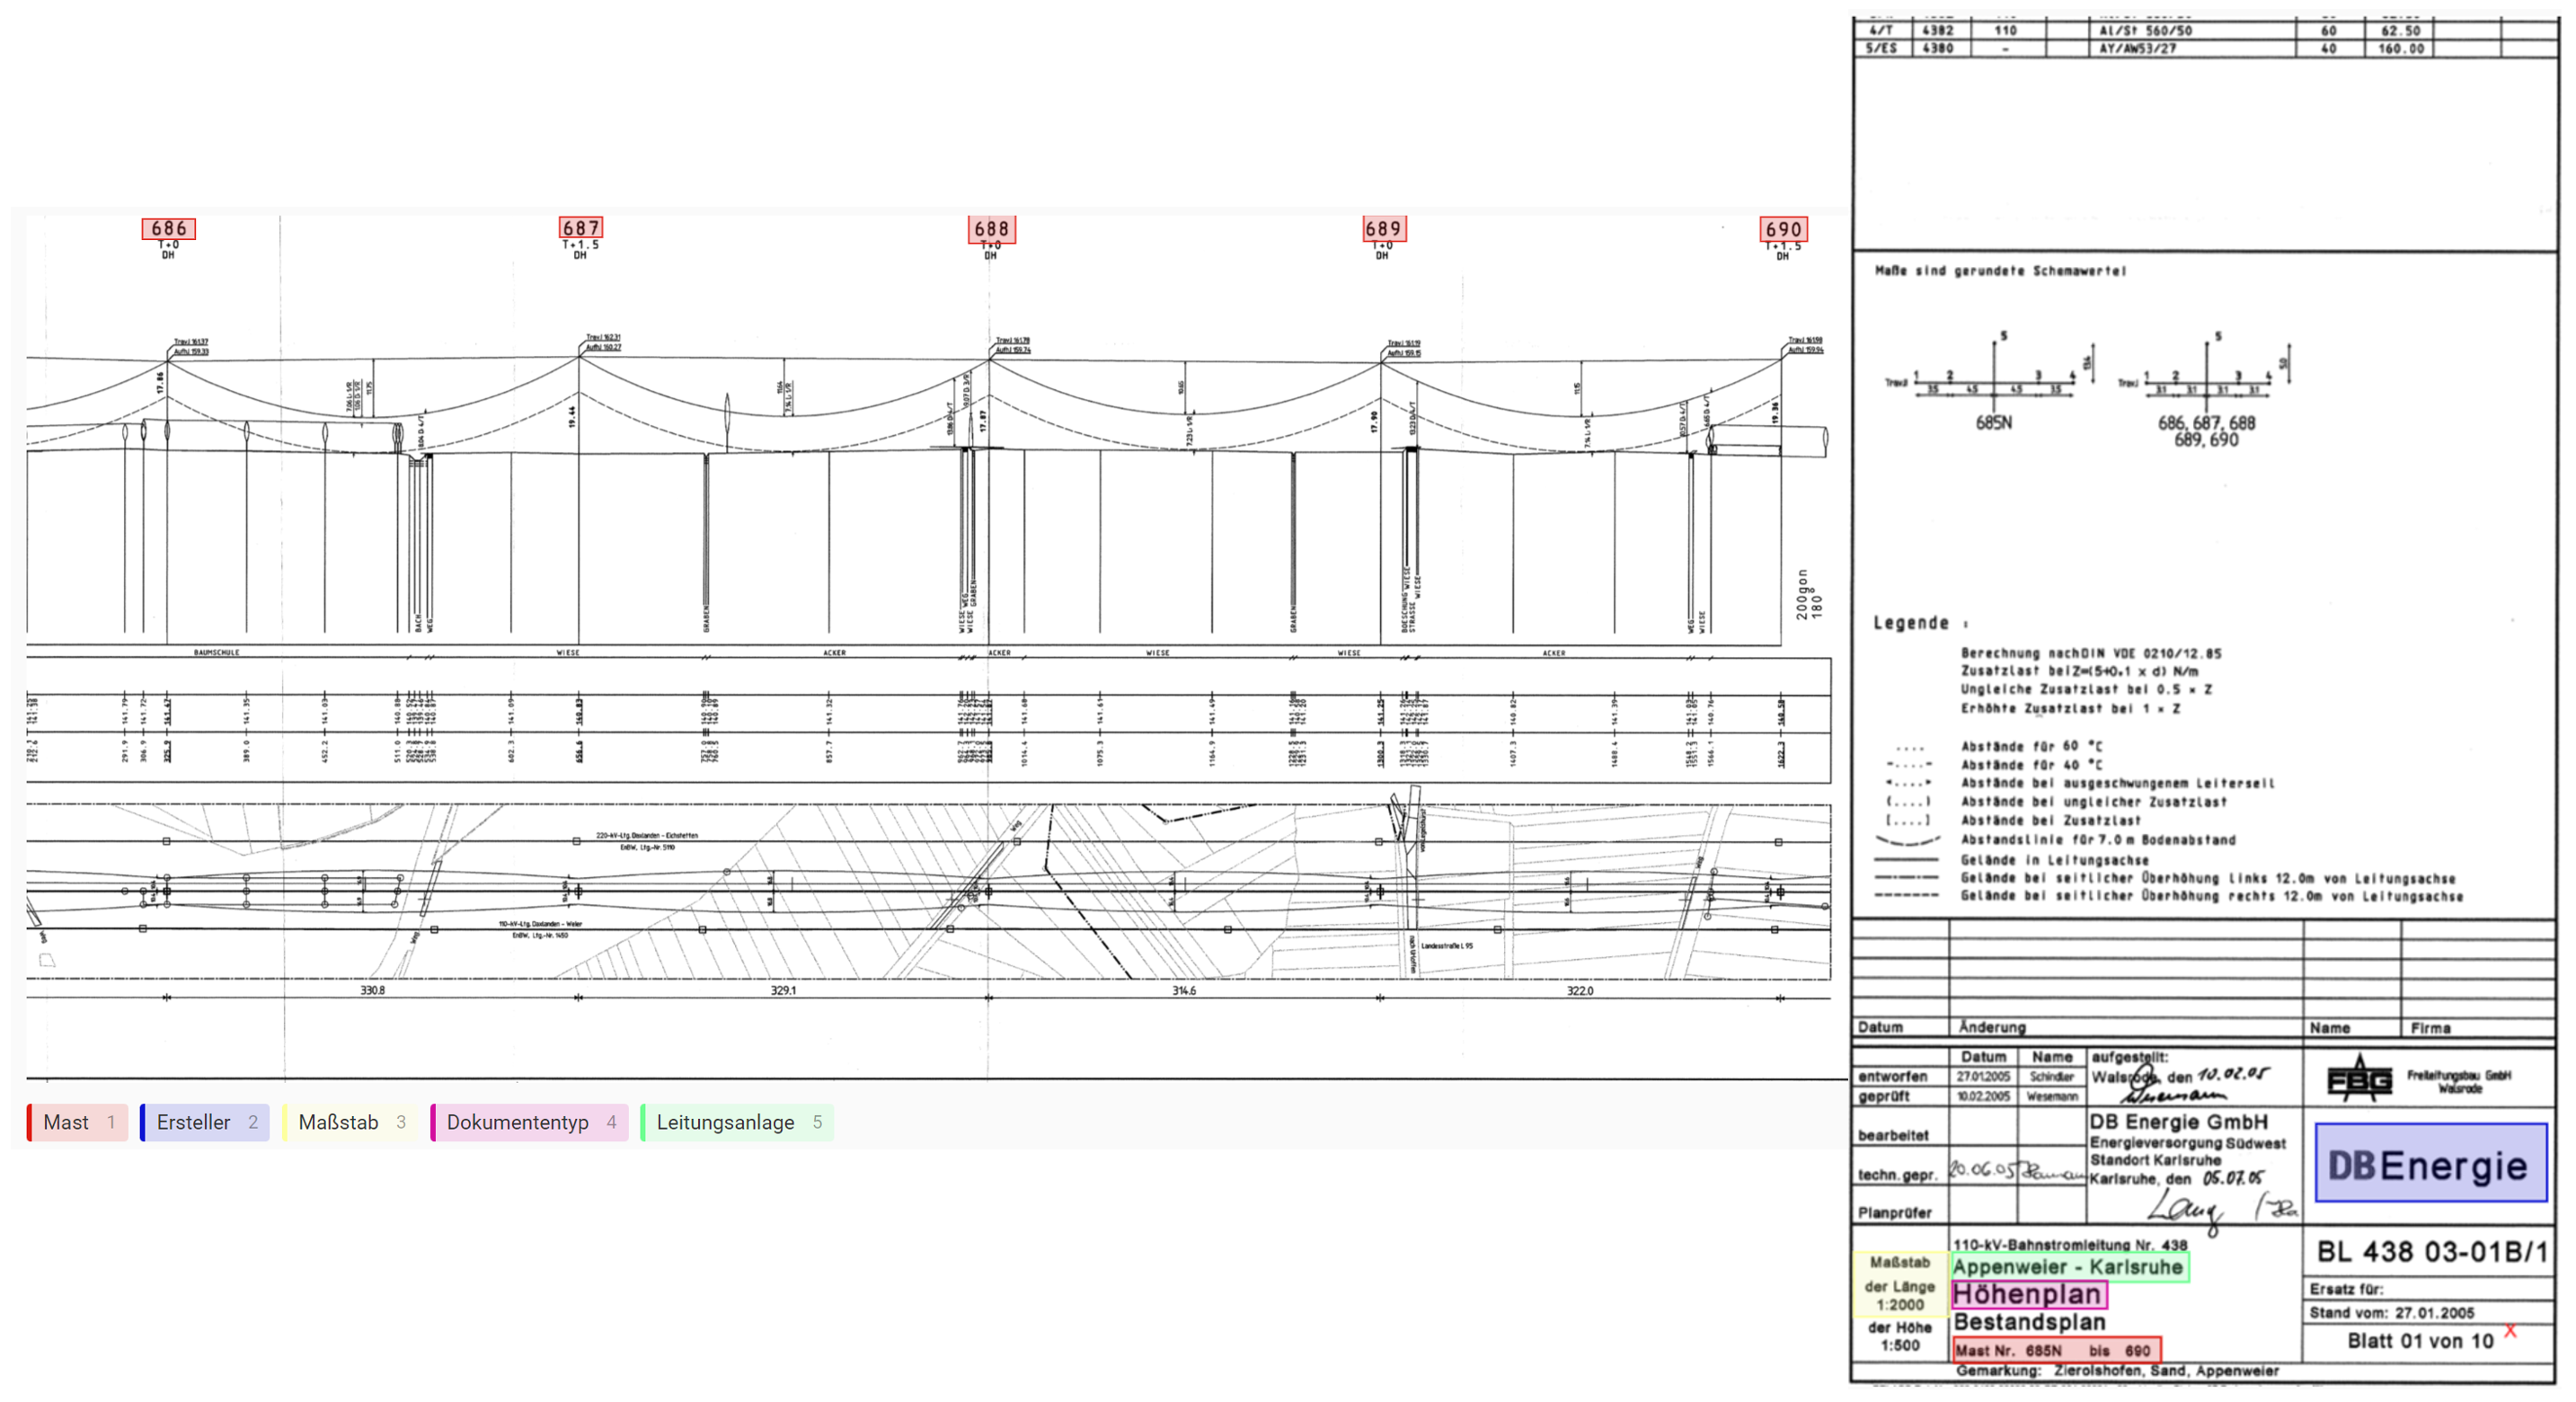
\includegraphics[width=1.0\linewidth]{DOKUMENT-Metadaten-Beispiel-2.png}
    \caption{Beispiele für die einzelnen Metadaten exportiert aus Label Studio}
    \label{fig:enter-label}
\end{figure}

\subsection{Aufbereitung der Daten}
%Hier werden die Schritte zur Vorbereitung und Anpassung der Daten für die Verarbeitung mit Donut und LayoutLM beschrieben.
Ziel ist die Erstellung eines sogenannten goldenen Datensatzes, der sowohl von Donut als auch von LayoutLM genutzt und auf HuggingFace hochgeladen werden kann, um eine geräteunabhängige Nutzung zu ermöglichen.

\subsubsection{Anforderungen der Modelle}
Die beiden Modelle, Donut und LayoutLM, stellen unterschiedliche Anforderungen an die Struktur der Daten. Donut soll im Rahmen des Document Visual Question Answering (DocVQA) eingesetzt werden, um Metadaten durch gezielte Prompts effizient zu extrahieren. Dies erfordert eine Datensatzstruktur, die keine Bounding-Box-Informationen benötigt, wie im folgenden Beispiel illustriert:
\begin{lstlisting}[language=json,firstnumber=1]
{'file_name': 'image', 'ground_truth': {'gt_parses': 
[{'question': 'Was ist der Ersteller?', 'answer': 'Firma X'}]}}
\end{lstlisting}
Im Gegensatz dazu benötigt LayoutLM eine Datenstruktur, die das BIO-Format verwendet, in dem Klassen durch Zahlen repräsentiert und die gefundenen Wörter diesen Klassen zugeordnet werden:
\begin{lstlisting}[language=json,firstnumber=1]
{"file_name": "image", "tokens": ["EQOS Energie", "Daxlanden - Weier", "Baugrunderkundung"], 
"bboxes": [[1267, 998, 1364, 1015], [1017, 1027, 1144, 1044], [134, 149, 368, 175]], 
"ner_tags": [0, 1, 2]}
\end{lstlisting}

\subsubsection{Labeling für Donut}
%pdf->image Boundingbox -> bbox
Für das Training der Modelle waren Bilder anstelle von mehrseitigen PDFs erforderlich, was eine Konvertierung der Dokumente notwendig machte. Eine besondere Herausforderung stellte die Umwandlung der Bounding-Boxen dar, da diese in den ursprünglichen PDFs als feste Pixelkoordinaten vorlagen. Die Koordinaten mussten in das Format(xmax,xmin,ymax,ymin) in relativer Position zur Größe des bildes überführt werden. Zudem waren ursprünglich einzelne Wörter durch Bounding-Boxen markiert, jedoch benötigte ich zusammenhängende Bounding-Boxen für korrekte Antworten. Daher wurden nahe beieinander liegende oder überlappende Bounding-Boxen zusammengefasst und der zugehörige Text verbunden.

Bei der Extraktion musste jede Seite einzeln bearbeitet werden, wobei in der Regel nur die erste Seite gelabelt war, was zur Folge hatte, dass nachfolgende Seiten verworfen wurden. Ebenso wurden Dokumente ohne Labeling ausgeschlossen.\\
%text,prompt -> ground_truth
Um die ground\_truth zu erstellen, implementierte ich ein Prompt-Feld, das das gesuchte Label speichert und daraufhin die Abfrage formuliert wird, sowie ein Text-Feld, das die korrekte Antwort enthält und als Vergleichsbasis für die Modellausgabe dient.

Zudem ergab sich eine weitere Herausforderung aus der Beschränkung, dass die ground\_truth pro Dokument lediglich einen einzigen Prompt zuließ, während mehrere Labels vorhanden waren und nach verschiedenen Metadaten gesucht werden sollte. Um dieses Problem zu bewältigen, wurden Kopien der Bilder erstellt, die mehrere Labels enthielten. Jeder Kopie eines Bildes wurde eine spezifische ground\_truth zugewiesen, die ein einzelnes Label enthielt. \\
%fill empty text
Um den Datenverlust insbesondere bei den Dokumenten, die zwar ein Label und eine Bounding Box, aber keine expliziten Textangaben aufwiesen, zu minimieren, wurde auf die vorhandenen OCR-Dateien zurückgegriffen. Diese Maßnahme diente der Rekonstruktion fehlender Textangaben, indem das Wort aus den OCR-Dateien extrahiert wurde, sofern es innerhalb einer festgelegten Toleranzgrenze von 0,004 Einheiten in der jeweiligen Bounding Box positioniert war. Dieser spezifische Spielraum wurde experimentell bestimmt, um ein optimales Gleichgewicht zwischen der Minimierung falsch zugeordneter Wörter und der Maximierung korrekt erkannter Wörter zu erreichen. 

Im Zuge der Implementierung stellte sich heraus, dass das Encoding der Bilder mittels Base64 zwar eine umfassende Lösung darbot, jedoch erhebliche Nachteile hinsichtlich der Verarbeitungszeit und des Speicherplatzverbrauchs mit sich brachte. Angesichts dieser Einschränkungen entschied ich mich für die Verwendung der Funktion load\_dataset("imagefolder") von HuggingFace. Diese Methode ermöglicht eine automatisierte Codierung der Bilder und das effiziente Verpacken der zugehörigen Metadaten in einem Datensatz.

Um diese Funktion nutzen zu können, war es erforderlich, eine metadata.jsonl-Datei zu erstellen, die für jedes Bild den entsprechenden Dateinamen sowie die zugehörigen Metadaten beinhaltete.\\ 
%Downscale images
Angesichts der hohen Qualität meiner Dokumente, die zum Teil aus umfangreichen .tiff-Bildern mit Dateigrößen von bis zu 38 MB bestanden, entschied ich mich, die Auflösung dieser Bilder um die Hälfte zu reduzieren. Diese Maßnahme zielte darauf ab, Probleme mit DOS-Fehlern zu vermeiden und die Trainingszeiten signifikant zu verkürzen. Trotz der Reduktion der Bildgröße und der damit verbundenen Pixelanzahl blieb die Punktdichte (DPI) konstant bei 96. Diese Konstanz ist von kritischer Bedeutung für die Leistungsfähigkeit der OCR-Erkennung und des Donut-Modells, da eine angemessene DPI-Zahl entscheidend für die Genauigkeit der Textextraktion aus den Bildern ist. Zudem resultierte diese Skalierung in einer mehr als doppelten Reduzierung des benötigten Speicherplatzes, was die Effizienz des gesamten Trainingsprozesses verbesserte.\\
%labeling von massstab (problem mit dateinamen)
In meiner Arbeit stellte sich heraus, dass der Maßstab, ein kritischer Metadatenwert, in den ursprünglichen Labels nicht enthalten war. Um diese Lücke zu schließen, entschloss ich mich, den Maßstab eigenhändig nachzutragen. Hierzu verwendete ich das Tool Label-studio, um den Maßstab in 83 Dokumenten manuell zu labeln und diese korrigierten Daten anschließend in meinen Datensatz zu integrieren.

Eine Herausforderung dabei war, dass die Dateinamen durch Label-studio beim ersten Labeling-Prozess automatisch modifiziert und gekürzt wurden, falls sie eine bestimmte Länge überschritten. Diese Modifikation führte dazu, dass ich die zugehörigen Labels nicht mehr eindeutig den entsprechenden Bildern zuordnen konnte. Aus diesem Grund war es erforderlich, den Labeling-Prozess zu wiederholen, um sicherzustellen, dass die Daten korrekt und nachvollziehbar in den Datensatz eingefügt werden konnten.\\
% Train/Test split erklart
Im Rahmen meines Ansatzes erhielt ich für das Modell Donut einen Datensatz von insgesamt 1365 Dokumenten. Diesen Datensatz teilte ich in 95\% Trainingsdaten und 5\% Testdaten auf. Die Entscheidung für einen derart kleinen Testdatensatz basierte auf der Überlegung, dass eine maximale Nutzung der verfügbaren Daten für das Training es ermöglicht, umfassendere Lernerfahrungen zu sammeln und die Modellgenauigkeit zu verbessern. Darüber hinaus ermöglicht die Verwendung der nicht gelabelten Bilder für zusätzliche Tests eine weiterführende Bewertung des Modells. Allerdings erfordert dies eine manuelle Überprüfung der Ausgaben, was den Validierungsprozess zeitintensiver gestaltet.

\subsubsection{Labeling für LayoutLMv3}
\paragraph{Phase 1: Anpassung der Datenstruktur}
Zunächst nutzte ich denselben Datensatz, der auch für das Modell Donut verwendet wurde. Die ursprünglichen Prompts unter der Rubrik GroundTruth wurden in NER-Tags umgewandelt. Die korrekten Antworten, die zuvor als Text unter GroundTruth aufgeführt waren, wurden in die Spalte Tokens überführt. Die Umwandlung sah wie folgt aus:
\begin{lstlisting}[language=json,firstnumber=1]
{'Ersteller': 0, 'Leitungsanlage': 1, 'Dokumenttyp': 2,  'Mast': 3, 'Maßstab': 4}
\end{lstlisting}
Zusätzlich mussten die Bounding-Boxen angepasst werden. Diese wurden zu festen Pixelkoordinaten umgewandelt, die den Größen der herunterskalierten Bilder entsprachen.\\
Beispielspalte des Datensatzes:
\ref{sec:Phase1}



\paragraph{Phase 2: Konsolidierung der Dokumente}
Im zweiten Schritt machte ich die Aufteilung in ein Label pro Dokument rückgängig und führte die Kopien wieder zusammen. Dadurch reduzierte sich die Gesamtanzahl der Dokumente, jedoch enthielt jedes Dokument nun mehrere Tokens und NER-Tags. Diese Tags waren nicht immer vollständig, da beim Labeln häufig eines oder mehrere vorhandene Labels weggelassen wurden.\\
Beispielspalte des Datensatzes:
\ref{sec:Phase2}



\paragraph{Phase 3: Einführung des Labels 'Other'}
Im dritten Datensatz wurde das Label 'Other': 5 eingeführt, um jedes Wort, das noch keinem Label zugeordnet war, entsprechend zu kennzeichnen. Um dem Problem unvollständig gelabelter Dokumente entgegenzuwirken, wurde eine Liste aller als Label klassifizierten Token erstellt und jedes gefundene Wort mit dieser Liste verglichen. Worte, die in der Liste enthalten waren, wurden entsprechend gelabelt, alle anderen als 'Other' eingestuft. Diese Vorgehensweise sollte Konsistenz in der Labelzuweisung gewährleisten, zum Beispiel, dass 'EQOS' durchgängig als 'Ersteller' und nicht als 'Other' gekennzeichnet wurde.

Um die Wörter selbst zu extrahieren, wurden zunächst die vorhandenen OCR-Dateien genutzt, jedoch stellte sich heraus, dass dies zu unbefriedigenden Ergebnissen führte, da der LayoutLMv3-Prozessor im Hintergrund Tesseract OCR (Englisch) verwandt, was oft zu abweichenden Wörtern führte, zum Beispiel wurde 'ü' zu 'ii'. Daher wurde zu hOCR Tesseract gewechselt, um ähnliche OCR-Fehler zu produzieren, die anschließend gemappt wurden. So konnte beispielsweise 'Kühmoos' nur als 'Kiihmoos' erkannt werden, dieses war dann jedoch aufgrund des eigenen hOCR Fehlers auch als 'Leitungsanlage' eingetragen und wurde von LayoutLM auch so erkannt.\\
Beispielspalte des Datensatzes:
\ref{sec:Phase3}

\section{Implementierung}
\subsection{Anwendung von Donut}
%Diese Sektion zeigt, wie das Modell Donut zur Dokumentenverarbeitung eingesetzt und angepasst wird.
Nachdem ein geeigneter Datensatz für das Donut-Modell zusammengestellt wurde, erfolgte die Konfiguration der Modellparameter, um eine optimale Verarbeitungsleistung zu gewährleisten. Die Bildgröße wurde auf 1280x960 Pixel eingestellt, was der Auflösung der meisten Dokumente im Datensatz entspricht. Die maximale Token-Länge wurde auf 128 festgelegt, was ausreichend ist, um die längsten erwarteten korrekten Antworten vollständig darzustellen und eventuelle Fehler in den Modellausgaben effektiv zu erkennen.

Für das Training wurde das vortrainierte Modell naver-clova-ix/donut-base \cite{DONUT-donut-base} verwendet. Um die Trainingseffizienz zu erhöhen, wurden spezifische Tokens wie „Leitungsanlage“, „Mast“, „Massstab“, „Ersteller“, „Dokumentenart“ und „Dokumenttyp“ von Anfang an in den Tokenizer integriert. Diese Maßnahme verhinderte, dass das Modell diese Begriffe während des Trainings selbst erkennen musste und stellte sicher, dass solche Begriffe als Ganzes erkannt wurden, ohne sie fälschlicherweise in Tokens wie „Mas t“ für „Mast“ oder „Er s teller“ für „Ersteller“ aufzuspalten.

Um eine einheitliche Dokumentengröße zu gewährleisten und das Training in Batches zu ermöglichen, wurde ein Padding von -100 angewendet.Ausserdem wurde Masking während des Trainings verwendet, um die Modellleistung weiter zu verbessern.

Das Training von Donut wurde über 30 Epochen mit jeweils 800 Dokumenten pro Epoche durchgeführt. Am Ende des Trainings wurde das Modell mit den Gewichten der besten Epoche gespeichert, um die optimale Leistung des Modells zu sichern.

\myworries{Es wäre auch möglich gewesen, alle korrekten Antworten als mögliche Tokens hinzuzufügen und die Funktion json2token anzupassen, um potenziell schne bessere Ergebnisse zu erzielen.}

\subsection{Ergebnisse von Donut}
Nach der Trainingsphase wurde Donut in seiner Grundkonfiguration mit den Testdaten evaluiert. Dabei wurden die tatsächlichen Daten (Ground Truth) direkt mit den Modellausgaben verglichen. Umlaute und das scharfe S (ö, ä, ü, ß) wurden zu ihren entsprechenden englischen Äquivalenten gemappt, um Fehlerquellen zu minimieren.

\begin{figure}[H]
    \centering
    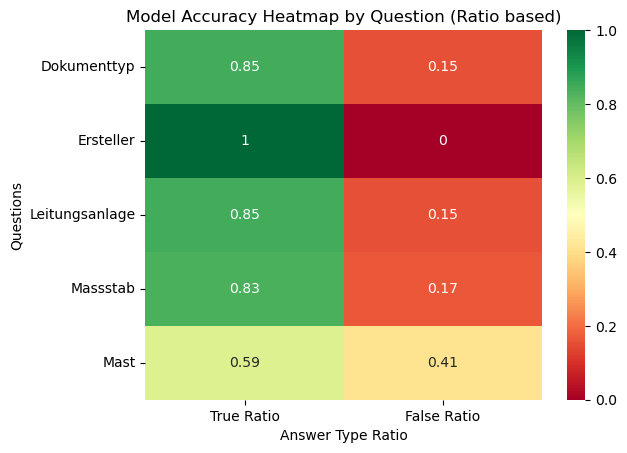
\includegraphics[width=0.5\linewidth]{DONUT-Transformer-results.png}
    \caption{Ergebnisse von Donut nach 30 Trainings-Epochen}
    \label{fig:enter-label}
\end{figure}

Die Gesamtwahrscheinlichkeit, ein Dokument korrekt zu klassifizieren, wurde wie folgt berechnet: \(0.85 \times 1 \times 0.85 \times 0.83 \times 0.59 = 0.35\), da alle Parameter korrekt sein müssen, um einen korrekten Dateinamen zu vergeben.

\subsubsection{Haufige Fehler}
\begin{table}[H]
\centering
\caption{Comparison of Ground Truth and Model Answers}
\begin{tabular}{|>{\raggedright\arraybackslash}p{8cm}|>{\raggedright\arraybackslash}p{5cm}|}
\hline
\textbf{Ground Truth} & \textbf{Model Answer} \\ \hline
\textbf{Dokumenttyp:} &  \\
Fundamentstatik & Statische Berechnung \\
Bauablaufschema & Bauablaufplan \\ \hline

\textbf{Ersteller:} &  \\ \hline

\textbf{Leitungsanlage:} &  \\
RDK Offenburg & Daxlanden Eichstetten \\
Daxlanden-Eichstetten & Daxlanden-Eichsteten \\
Daxlanden - Eichstetten & Daxlanden - Elchstetten \\
Daxlanden Eichstetten Daxlanden Weier  & Daxlanden Eichstetten \\ \hline
Weier UW Eichstetten & Weer - Eichatitan \\
\textbf{Maßstab:} &  \\
Maßst.: 1:20 & Maßst.: 1:15 \\ \hline

\textbf{Mast:} &  \\
1017 & 1016 \\
194A & 188A \\
817A & 1012A \\
474A & 561A \\
13 & 122 \\
474a & von474abis479a \\
008 & von008bis012 \\
Von 114 bis 120 & 1023 \\ \hline
\end{tabular}
\end{table}

Häufige Fehler umfassten die Verwechslung von I und L, das Fehlen eines Buchstabens oder die semantische Übereinstimmung mit der Ground Truth unter Verwendung eines Synonyms, das ebenfalls im Dokument zu finden war. Besonders problematisch war das Modell bei Zahlen, da sowohl beim Maßstab als auch bei der Mastnummer oft Zahlen erbracht wurden, die nicht im Dokument zu finden waren. Ein weiteres Problem war das korrekte Auffinden von von-bis Mastnummern, die jedoch nicht in der Ground Truth standen.

\subsection{Mapping von Donut auf vorhandene Metadaten}

Um die Ergebnisse besser einschätzen zu können, wurde zunächst eine genaue Übersicht über die Anforderungen erstellt. Insbesondere bei den Dokumenttypen wie Lageplan 1:2500 (IHL), Lageplan mit Schutzgebieten 1:2500 (IHL) und allgemeinem Lageplan war es wichtig, diese zunächst richtig als Lagepläne zu erkennen. Später konnte dann anhand des Maßstabes eine Feinunterscheidung zwischen den verschiedenen Lageplänen vorgenommen werden. Bei dieser Feinunterscheidung ist der Maßstab nur in 6 von 230 Fällen für die Erkennung des Dokumenttyps notwendig. Da der Maßstab zunächst nicht von großer Bedeutung war, konnte die Genauigkeit des Maßstabs bei der Berechnung zunächst vernachlässigt werden. 
\myworries{Vielleicht hier das zunachst streichen. Und dann meine eigene Dokumentklassifikation Introducen}

Für den Auftraggeber ist es auch wichtig zu erkennen, ob ein Dokument von Donut falsch klassifiziert wurde. Dies kann durch den Konfidenzwert beurteilt werden, der durch den Parameter \texttt{output\_scores=True} bei der Generierung von der Antwort von Donut erzeugt wird.

Die von der Firma zur Verfügung gestellte Liste „EPLASS Plannummernkonvention” enthält alle möglichen Werte zu jedem Metadatum. In einem weiteren Schritt wurde versucht, das gefundene Ergebnis auf diese möglichen Metadaten abzubilden und das ähnlichste zu finden, um Fehler wie fehlende Buchstaben auszugleichen.

In einem erneuten Test wurden sowohl die Ground Truth als auch der Modelloutput mit allen möglichen Metadaten verglichen und das ähnlichste ausgewählt. Dies wurde mit der Ähnlichkeitssuche von Fuzzyfind \cite{Fuzzywuzzy} durchgeführt. Die beiden ähnlichsten Metadaten des Outputs und der Ground Truth wurden dann verglichen, was zu einer weiteren True/False-Aussage führte.
\myworries{HIer fuzzywuzzy medium beitrag zitieren oder referenz zu eigener Erklarung im Anhang z.B.?}

Eine neue Kategorie wurde hinzugefügt: Unsafe True und Unsafe False.  Jedem extrahierten Metadatum wurde ein Konfidenzintervall zugeordnet. Wenn die Konfidenz des aus dem Modell extrahierten Metadatums unterhalb dieses Konfidenzintervalls lag, wurde es als Unsafe klassifiziert. Anschließend wurde getestet, ob die Klassifizierung korrekt gewesen wäre, und je nach Ergebnis als Unsafe False oder korrekt als Unsafe True vermerkt.


\begin{figure}[H]
    \centering
    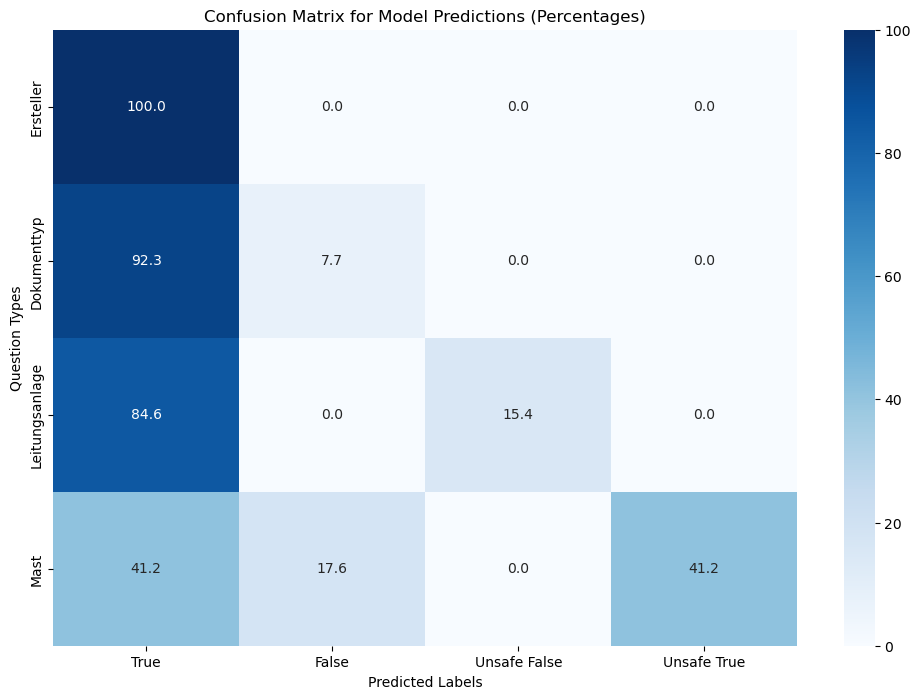
\includegraphics[width=0.7\linewidth]{DONUT-Transformer-results-unsafe.png}
    \caption{Ergebnisse nach mappen durch fuzzyfind}
    \label{fig:enter-label}
\end{figure}


Die angenommene korrekte Erkennungsrate nach Aussortierung der als False oder Unsafe markierten Dokumente beträgt \(1 \times 0.923 \times 0.846 \times 0.412\). Dabei haben sich alle Erkennungswerte der Metadaten verbessert, mit Ausnahme der Mastnummern, da hier kein einheitlicher Schwellenwert gefunden werden konnte, der die Konfidenz des Modells korrekt aufteilt. Um diesen großen Nachteil auszugleichen, sollte die Erkennung der Mastnummern durch LayoutLMv3 erfolgen.

\subsection{Anwendung von LayoutLM}
Das Training des LayoutLMv3-Modells wurde in drei aufeinander folgenden Phasen mit den in Abschnitt 3.2.3 beschriebenen Datensätzen durchgeführt. Die Trainingsparameter blieben in allen Phasen gleich und wurden wie folgt konfiguriert:

\begin{verbatim}
max_steps=1000,
per_device_train_batch_size=2,
per_device_eval_batch_size=2,
learning_rate=1e-5,
evaluation_strategy="steps",
eval_steps=100,
load_best_model_at_end=True,
metric_for_best_model="f1"
\end{verbatim}

Die Varianz im Training resultierte ausschließlich aus den spezifischen Strukturen der verwendeten Datensätze. Im ersten Trainingslauf wurde der Datensatz aus Phase 1 verwendet. Ein wesentliches  Problem bei diesem Ansatz war, dass das getestete Modell konsequent nur eine einzelne Bounding Box mit Label pro Gesamtdokument ausgab, obwohl diese durchweg korrekt war. Es war nicht möglich, eine methodische Lösung zu entwickeln, die Vorhersagen für andere Labels innerhalb desselben Dokuments ermöglicht hätte. Eine Analyse der Logits zeigte, dass nur die NER-Tags des tatsächlich vorhergesagten Labels vorhanden waren.

Für das zweite Training wurde der Datensatz aus Phase 2 verwendet, welcher mehrere Labels pro Dokument enthielt und frei von Dokumentduplikaten war. Allerdings waren nicht alle Wörter gelabelt, und es fehlte das Label 'Other' für nicht zugehörige Wörter. Es wurde erwartet, dass das Modell nicht gelabelte Wörter eigenständig erkennen und entsprechend nur die erkannten Labels ausgeben würde. Dennoch gab das Modell mehrere Bounding Boxen mit Labels pro Dokument zurück, allerdings nicht in der erforderlichen Vollständigkeit. Dieser Trainingsansatz erwies sich als unzureichend, da nicht sichergestellt werden konnte, dass essenzielle Labels wie 'Mast' erkannt und zurückgegeben wurden, auch wenn andere Labels überflüssig waren.

In der dritten Trainingsphase wurde ein vollständig gelabelter Datensatz eingeführt und um das Label 'Other' ergänzt. Dieses Vorgehen erwies sich als erfolgreich: Das Modell lieferte nun für jedes Token eine Bounding Box mit dem entsprechenden Label.

\subsection{Ergebnisse von LayoutLM}

% Erklärung von Inference vs. True Inference
Beim Testen der Genauigkeit von LayoutLM ist es wichtig, zwischen verschiedenen Inferenzmodi zu unterscheiden. Man unterscheidet zwischen dem Standard Inference Modus, bei dem Dokument, Bounding Boxes, Labels und die Wörter selbst übergeben werden müssen, und dem True Inference Modus. Bei letzterem wird lediglich das Dokument übergeben. Das Modell wurde ausschließlich im True Inference Modus getestet, da auch in Zukunft keine OCR-Daten standardmäßig mitgeliefert werden. In diesem Modus wird das Dokument nochmals mittels OCR verarbeitet, wobei OCR-Fehler bewusst in die Fehleranalyse des Modells einbezogen werden. Dies dient nicht der Bewertung der alleinigen Modellleistung, sondern der Überprüfung der tatsächlichen Genauigkeit, mit der Labels extrahiert werden können.


\begin{figure}
    \centering
    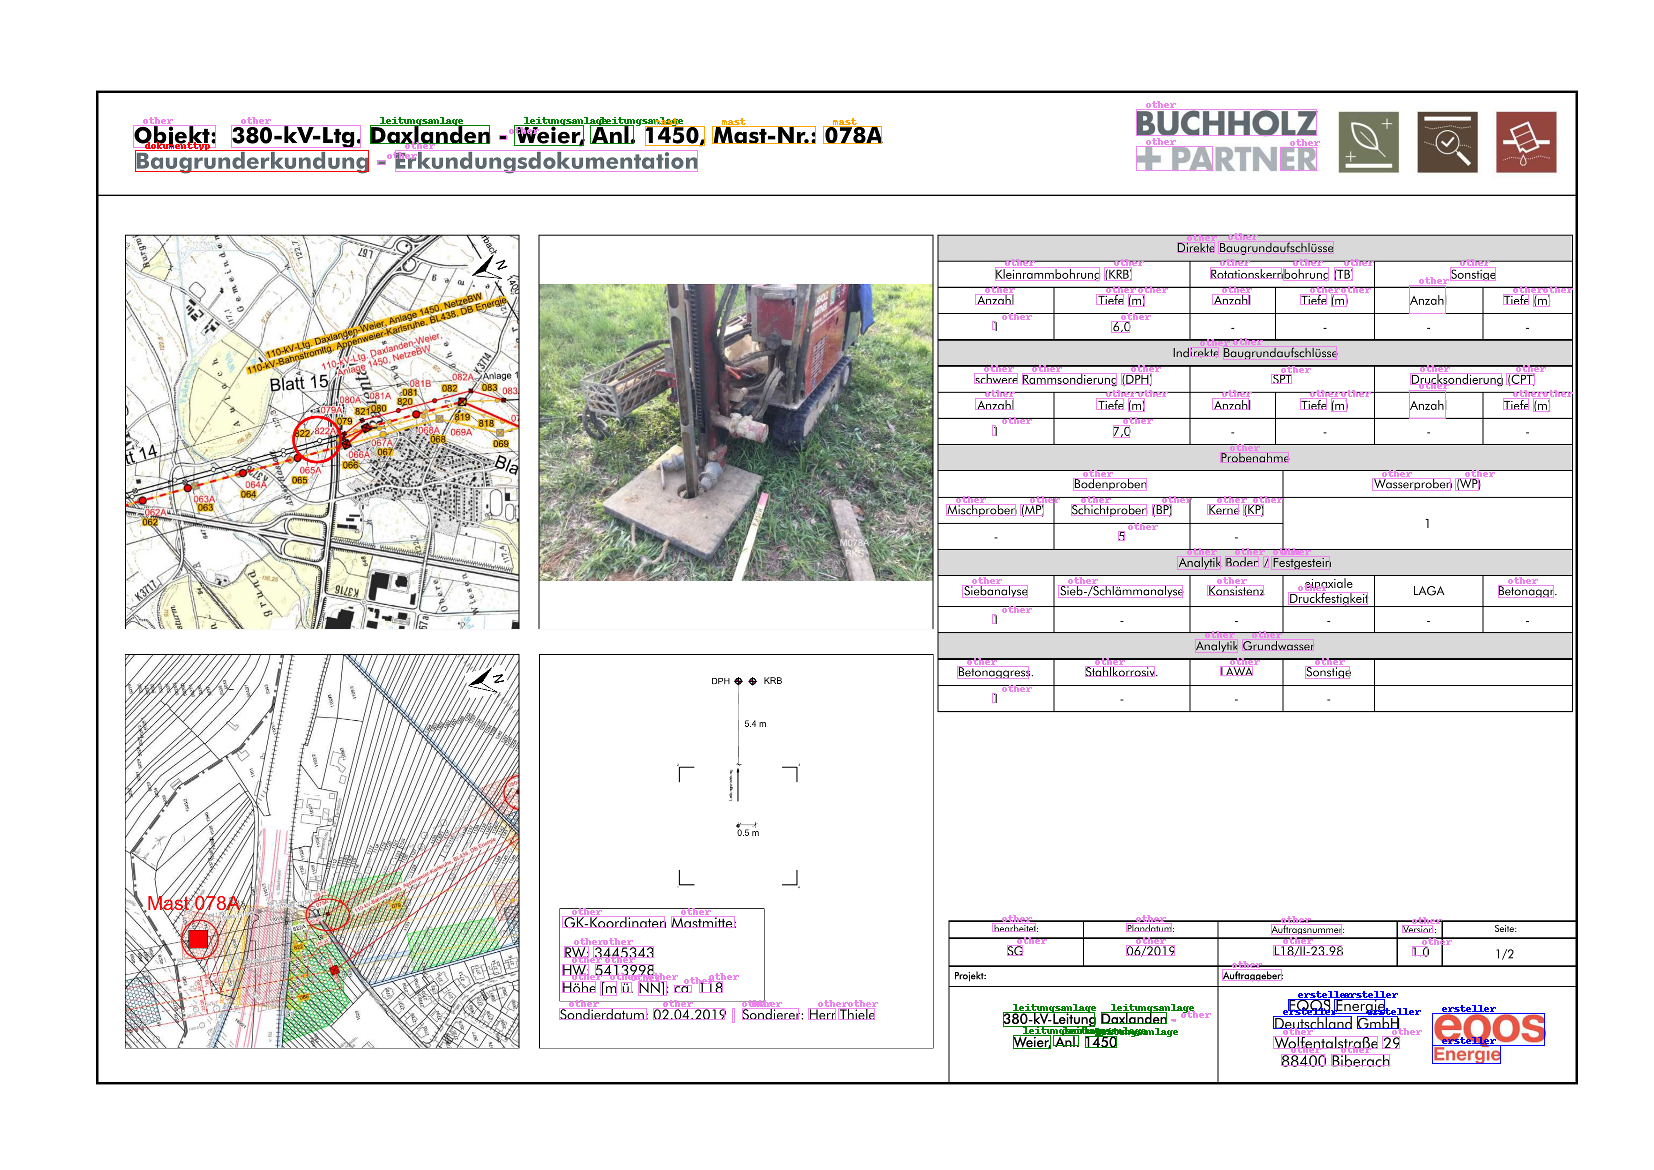
\includegraphics[width=0.9\linewidth]{LayoutLMv3-results.png}
    \caption{Beispiel fur die Finale Ausgabe von LayoutLMv3}
    \label{fig:enter-label}
\end{figure}
Um die Metadaten aus dem Dokument zu extrahieren, wurden die einzelnen Bounding Boxen um 4 Pixel in alle Richtungen vergrößert, um ein Abschneiden von Buchstaben zu vermeiden und aus dem Dokument ausgeschnitten. Anschließend wurde jedes ausgeschnittene Bild mit EasyOCR gescannt. EasyOCR wurde aufgrund seiner nachweislich hohen Genauigkeit als Open-Source OCR-Tool ausgewählt, wie in \cite{Layoutlmv3-easyocr} dargelegt.

\begin{figure}[H]
    \centering
    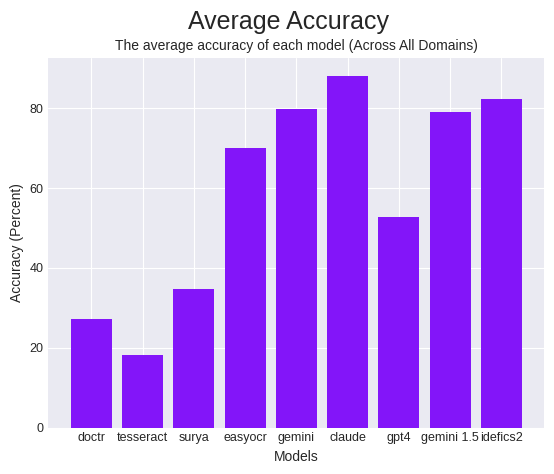
\includegraphics[width=0.5\linewidth]{LayoutLMv3-easyocr-comparisson.png}
    \caption{EasyOCR im Vergleich}
    \label{fig:enter-label}
\end{figure}

Die extrahierten Metadaten wurden mit der Ground Truth verglichen, wobei eine Genauigkeit von 78\% erreicht wurde. Bei der Berechnung dieser Genauigkeit wurden Fälle ausgeschlossen, in denen sowohl das erkannte Token als auch die Ground Truth als 'Other' klassifiziert wurden. Diese Fälle waren zahlreich vorhanden und hätten die Genauigkeit des Modells auf eine verzerrte Rate von 98\% erhöht. Um eine vergleichbare Bewertung mit dem Donut-Modell zu ermöglichen, wurden diese korrekt als 'Other' identifizierten Wörter nicht in die Genauigkeitsberechnung einbezogen.

\subsection{Kombinierter Einsatz von Donut und LayoutLMv3}
% Darstellung der Kombination beider Modelle zur Erzielung optimaler Ergebnisse.
In diesem Ansatz wurden die Stärken von Donut und LayoutLMv3 kombiniert, um optimale Ergebnisse zu erzielen. Zunächst verarbeitete das Donut-Modell das Dokument und gab die extrahierten Metadaten mit den zugehörigen Konfidenzwerten aus. Eine spezifische Verarbeitung wurde für die Kategorien 'Mast' und 'Dokumenttyp' durchgeführt. Für 'Dokumenttyp' wurde nach ähnlichen Dokumenttypen gesucht, um eine breitere Abdeckung zu gewährleisten und anschließend eine Feinabstimmung, z.B. auf Basis des Maßstabs, vornehmen zu können.

War die Konfidenz für 'Mast' zu gering, wurde die Aufgabe an LayoutLMv3 übergeben. Für die Verarbeitung durch LayoutLMv3 musste jedoch sichergestellt werden, dass die Dokumente nicht mehr als 512 Token enthielten, was in den meisten Fällen der Fall war. Um das Dokument dennoch adäquat verarbeiten zu können, wurde es in Abschnitte unterteilt und diese wurden einzeln an das LayoutLMv3-Modell übergeben. Dies geschah mit Hilfe eines Tokenizers, der das Dokument nach jeweils 512 Tokens segmentierte und zur Verarbeitung weiterleitete. Diese Methode erwies sich als effektiv, insbesondere weil die Mastnummer meist in einer einzigen Zeile stand und somit vollständig extrahiert werden konnte.
%\myworries{Ein Beispiel für ein solches Dokument einfügen}
\begin{figure}[H]
    \centering
    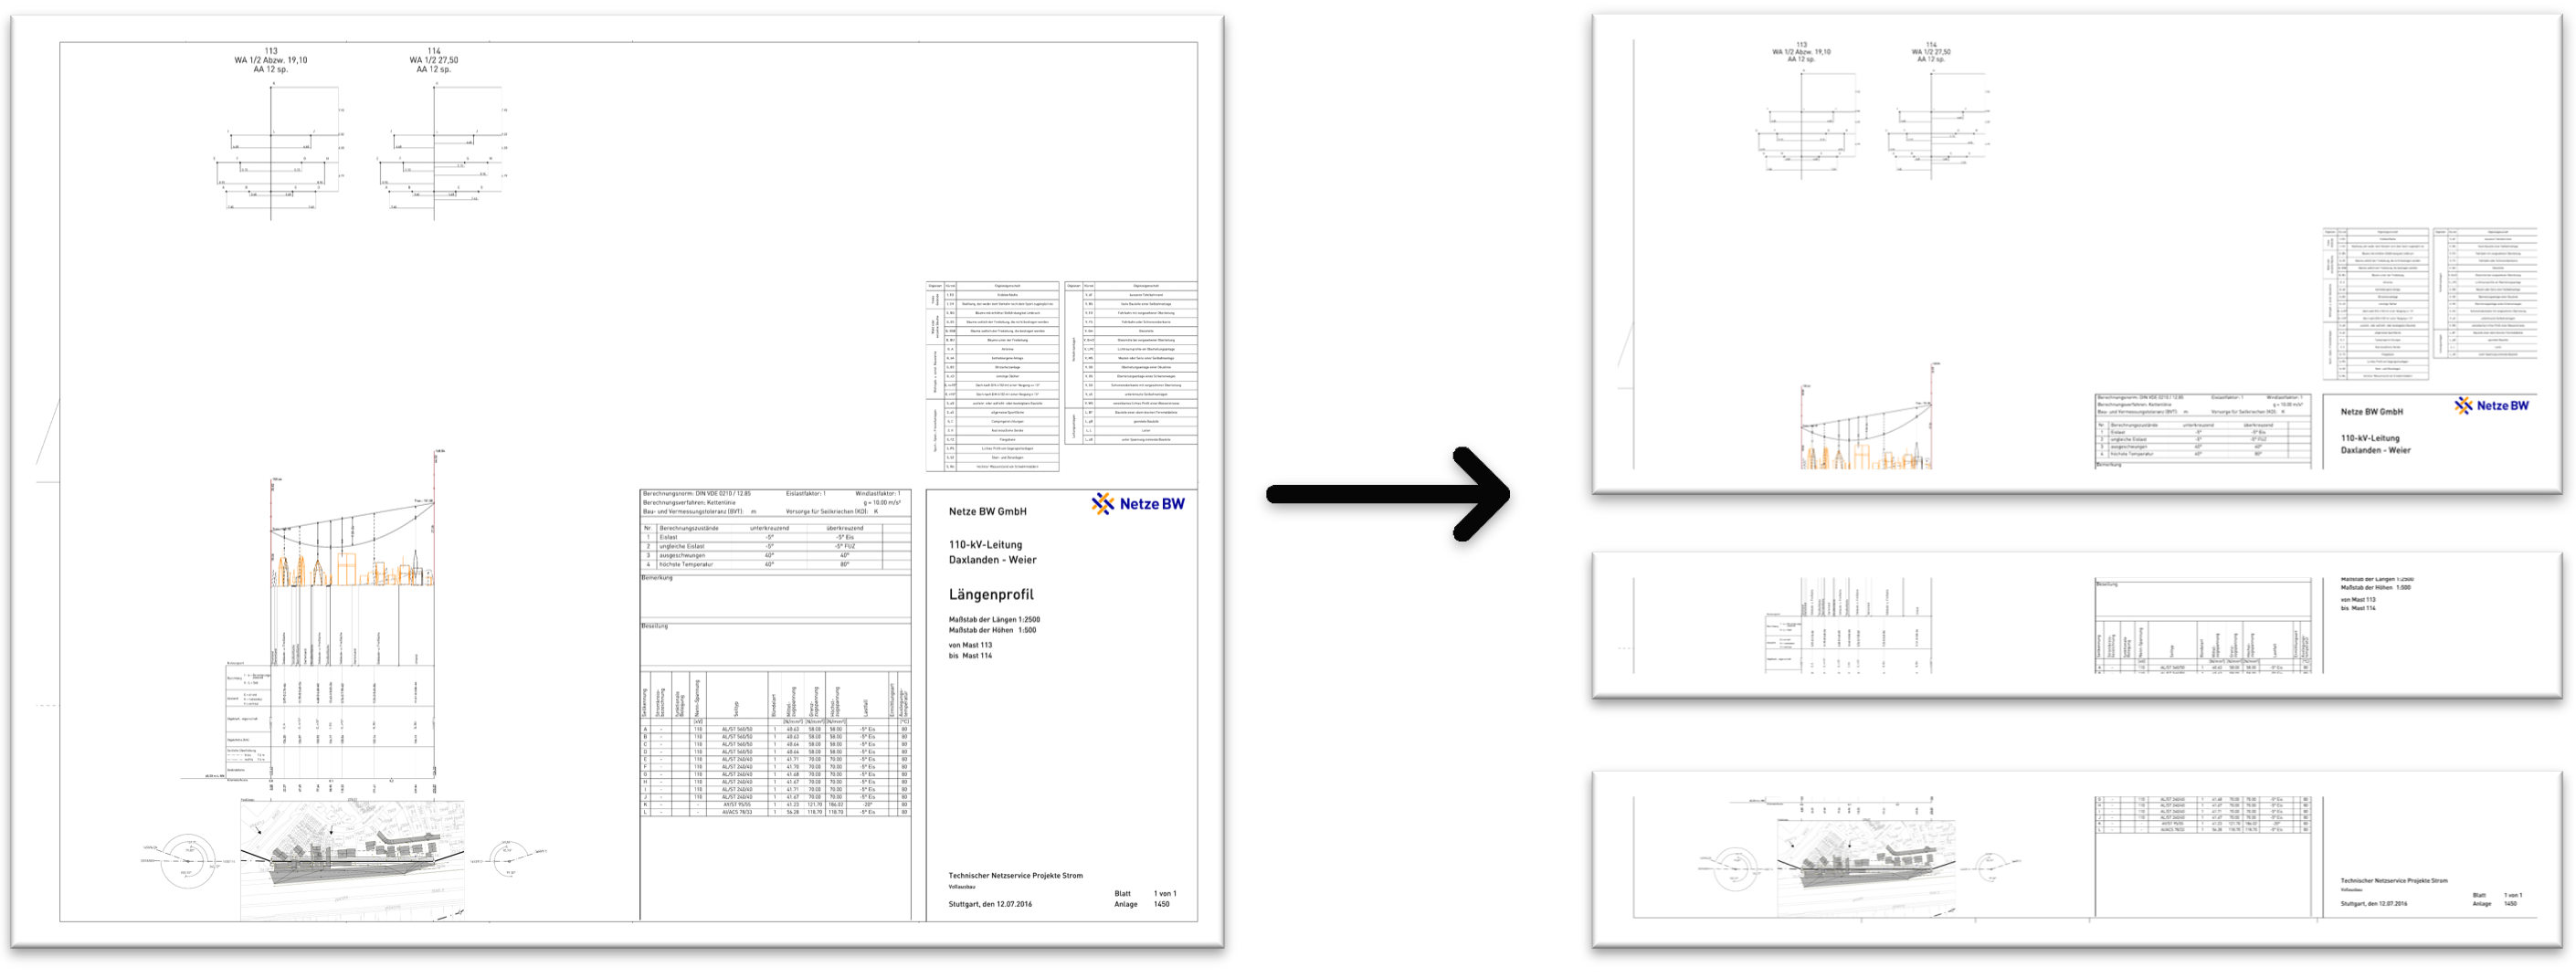
\includegraphics[width=1.0\linewidth]{DOKUMENT-Segmentation-Horizontal.png}
    \caption{Darstellung einer Dokumentzerteilung nach 512 Token}
    \label{fig:enter-label}
\end{figure}


\section{Diskussion}
% Präsentation und Diskussion der Ergebnisse der durchgeführten Experimente und Tests.
Die Integration beider Modelle resultierte in einer durchschnittlichen worst-case Genauigkeit von 64,3\% für die korrekte Klassifikation eines einzelnen Dokuments, berechnet als \(1 \times 0.923 \times 0.846 \times 0.823\). In anderen Fällen wurde deutlich, welches Metadatum wahrscheinlich inkorrekt klassifiziert wurde.

\section{Zusammenfassung und Ausblick}
\subsection{Haupterkenntnisse}
Zusammenfassung der wichtigsten Erkenntnisse aus der Arbeit.

\subsection{Herausforderungen und Limitationen}
Die Anwendung und Weiterentwicklung der Modelle im Rahmen dieser Forschungsarbeit hat mehrere Herausforderungen und Einschränkungen aufgezeigt, die sowohl die Ergebnisse als auch die praktische Umsetzung beeinflussen. Eine wesentliche Herausforderung ist die Erkennung falscher Mastnummern durch das LayoutLM-Modell. Dieses Problem tritt besonders häufig auf, da LayoutLM dazu neigt, Zahlen fälschlicherweise als Mastnummern zu identifizieren, was zur Notwendigkeit führt, spezielle Token wie "Mast" oder "Nr" zu erkennen und die Bounding Box entsprechend zu erweitern, um genauere Ergebnisse zu erzielen.

Außerdem werden tatsächlich alle Mastnummern gefunden, auch die, die nicht in der Ground Truth enthalten sind, was das Testen von LayoutLMv3 sehr erschwert, teilweise müssen die Testergebnisse noch manuell verifiziert werden.

Weiterhin zeigt sich, dass LayoutLM mit gescannten, alten oder handgeschriebenen Dokumenten deutlich schlechter zurechtkommt. Darüber hinaus wurde festgestellt, dass es häufige Fehler in den Datensätzen gibt. Einige dieser Fehler wurden bereits identifiziert, aber es besteht eine hohe Wahrscheinlichkeit, dass weitere unentdeckt bleiben. Ein besonderes Problem ist die fehlerhafte Zuordnung von Metadaten, bei denen z.B. die Bounding Box über das gesamte Dokument gezogen wurde, was die Verarbeitung erschwert und zu Ungenauigkeiten führt.

Des Weiteren ist die Genauigkeit des Other Labeling im dritten LayoutLMv3-Datensatz aufgrund von OCR-Fehlern sehr ungenau, was zu einer hohen Rate an Fehlklassifikationen führt. Schwierig ist auch die Klassifikation von Dokumenten anhand von Begriffen, die nicht im Dokument vorkommen, wie zum Beispiel "Ankerskizze". Hier wäre ein separates Training nur auf den Dokumenttyp notwendig.

Ein weiteres Problem ist das unvollständige EPLASS-Vergleichsdokument, bei dem Vergleiche fehlschlagen, obwohl das Metadatum korrekt erkannt wurde. Dieses sollte von der Arbeitgeberseite vervollständigt werden.

Außerdem sind die Dokumentnamen oft sehr lang und in einem falsch kodierten Format, was oft zu einer falschen oder verkürzten Konvertierung in UTF-8 führt. Dies ist besonders unpraktisch, da alle Dateiinformationen im Dateinamen gespeichert sind, was die Handhabung erschwert.

Diese Herausforderungen sind entscheidend für eine gezielte Optimierung, aber wenn diese Fehler behoben werden, kann die Extraktionsrate noch deutlich über 64\% gesteigert werden.

\subsection{Zukünftige Forschung}
Zukünftige Forschung in diesem Bereich sollte sich auf mehrere Schlüsselaspekte konzentrieren, um die Leistungsfähigkeit und Anwendbarkeit von Dokumentenanalysemodellen weiter zu verbessern. Ein wichtiger Schwerpunkt ist die bessere Zerlegung von Dokumenten. Die Entwicklung fortgeschrittener Techniken zur Segmentierung von Dokumenten kann dazu beitragen, die Genauigkeit der Textextraktion und -klassifikation erheblich zu verbessern. Insbesondere die genauere Identifizierung und Isolierung von Textblöcken, Bildern und anderen relevanten Elementen würde die Verarbeitungsqualität verbessern und könnte durch tiefer gehende neuronale Netze oder verbesserte heuristische Algorithmen erreicht werden.

Ein weiterer vielversprechender Ansatz ist die Anwendung des UDOP-Modells (Universal Document Processing).
\myworries{Kurz erklären}

Ein weiterer vielversprechender Ansatz ist die Anwendung von Donut Heatmaps (Deprecated).
\myworries{Hier einfugen dass nicht moglich weil model trainiert auf huggingface modelcode und nciht auf dem originalen und huggingface 'schlecht' implementiert - auf blogpost eingehen und verlinken und erklaren dass man dadurch die stellen der antworten sehen und mit OCR extrahieren koennte, alternative yu LayoutLMv3}

Darüber hinaus sollte besonderes Augenmerk auf die Anpassung des DONUT-Modells gelegt werden, um es speziell für die Klassifikation von Dokumenttypen zu trainieren. Dieser Ansatz könnte potenziell bessere Ergebnisse liefern, da er sich nur auf ein Metadatum konzentriert und die Kriterien, nach denen es klassifiziert, selbst festlegt, wodurch eine spätere Feinabstimmung und von Menschen erstellte Regeln, nach welchem Metadatum kategorisiert werden soll, wie z. B. des Maßstabes, überflüssig werden.
Dieser Ansatz wurde bereits in einem Versuch nach diese Bachelorarbeit umgesetzt, bei dem das DONUT-Modell ausschließlich auf die Erkennung und Klassifikation von Dokumenttypen trainiert wurde. Die Ergebnisse dieses Experiments waren vielversprechend, mit einer erreichten Genauigkeit von 84\%.

Ein weiterer wichtiger Forschungsbereich ist die Parallelisierung von Verarbeitungsprozessen. Durch den Einsatz moderner Hard- und Software kann die Geschwindigkeit der Dokumentenanalyse erheblich gesteigert werden. Die Implementierung asynchroner Verarbeitungsmethoden ermöglicht die gleichzeitige Verarbeitung mehrerer Dokumente, wodurch die Effizienz der Modelle in realen Anwendungen gesteigert werden kann.

\myworries{Andere Suchfunktion an stelle von FuzzyFind nutzen, auch strak auf Semantik eingehen}



\section{Anhänge}
\subsection{Beispiele}

\label{sec:Phase1}
\textbf{LayoutLMv3 Datensatzelement Phase 1}
\begin{lstlisting}[language=json,firstnumber=1]
{"id": "2899-ES-001b.png", "file_name": "2899-ES-001b_1.png", "tokens": ["Werkstattzeichnung"], "bboxes": [[4307, 3108, 4552, 3147]], "ner_tags": [2]}
\end{lstlisting}


\label{sec:Phase2}
\textbf{LayoutLMv3 Datensatzelement Phase 2}
\begin{lstlisting}[language=json,firstnumber=1]
{"id": "186953-413_D1_Index_03.png", "file_name": "186953-413_D1_Index_03.png", "tokens": ["D\u00e4mpfender Abstandhalter", "PFISTERER Switzerland AG"], "bboxes": [[818, 875, 1136, 908], [818, 1037, 1047, 1057]], "ner_tags": [2, 0]}
\end{lstlisting}


\label{sec:Phase3}
\textbf{LayoutLMv3 Datensatzelement Phase 3}
\begin{lstlisting}[language=json,firstnumber=1]
{'id': '000-0000-00000-00-QM-282-00010-01_TR-NSA-0050 Errichtung&nbsp; von Baustellenzaunen.png',
'file_name': '000-0000-00000-00-QM-282-00010-01_TR-NSA-0050 Errichtung&nbsp; von Baustellenzaunen.png', 
'tokens': ['transnet', 'bw', 'geltungsbereich:', 'transnetbw', 'gmbh', 'netzservice', 'arbeits-', 'und', 'gesundheits-', 'schutz', 'dokumentennumm:', 'tr-nsa-0050', 'version:', '4.1', 'vom', '08.01.2019', 'fachlich', 'zustandige', 'stelle:', 'tne', '~', 'projektentwicklung', 'bearbeiter:', 'herr', 'koch', 'technische', 'richtlinie', 'inkrafttreten:', '15.05.2019', 'klassifizierung:', 'inter', 'zur', 'externen', 'weitergabe', 'errichtung', 'von', 'baustellenzau-', 'zusammenfassung', 'hen', 'technische', 'richtlinie', 'zur', 'festlegung', 'von', 'temporaren', 'umzeunungen', 'bei', 'bautatigkeiten', 'beschlossen', 'durch', '/', 'am', 'herr', 'oehring', '09.05.2019', 'anlagen', 'keine', 'ppapierfassung', 'unteriiegt', 'nicht', 'dem', 'anderungscienst,', 'gltige', 'fassung', 'im', 'tng-intranet.'],
'bboxes': [[107, 116, 246, 137], [252, 120, 293, 137], [105, 167, 208, 181], [104, 201, 181, 211], [186, 201, 224, 211], [368, 135, 439, 145], [323, 160, 370, 170], [375, 160, 397, 170], [402, 160, 484, 170], [384, 176, 423, 186], [509, 110, 633, 120], [508, 134, 595, 144], [508, 168, 558, 178], [509, 201, 513, 211], [521, 201, 556, 211], [562, 201, 630, 211], [105, 234, 155, 244], [160, 234, 226, 247], [231, 234, 265, 244], [104, 268, 131, 278], [136, 274, 143, 275], [148, 268, 262, 281], [105, 301, 171, 311], [105, 334, 131, 344], [136, 334, 166, 344], [338, 284, 408, 294], [414, 284, 468, 294], [509, 234, 581, 244], [509, 268, 577, 278], [509, 301, 600, 314], [509, 334, 542, 344], [547, 337, 567, 344], [571, 335, 623, 344], [628, 334, 699, 347], [125, 388, 323, 425], [337, 395, 406, 417], [422, 388, 704, 417], [104, 626, 221, 639], [380, 440, 446, 462], [417, 626, 487, 636], [493, 626, 547, 636], [552, 629, 571, 636], [576, 626, 642, 639], [648, 629, 669, 636], [417, 643, 487, 655], [493, 642, 581, 655], [587, 642, 603, 652], [609, 642, 695, 655], [105, 769, 182, 779], [187, 769, 220, 779], [225, 769, 229, 779], [233, 771, 251, 779], [418, 769, 444, 779], [448, 769, 496, 782], [634, 769, 702, 779], [104, 802, 154, 815], [418, 802, 450, 813], [99, 1119, 169, 1129], [173, 1119, 218, 1129], [222, 1119, 245, 1127], [248, 1119, 269, 1127], [273, 1119, 356, 1129], [363, 1119, 395, 1129], [399, 1119, 440, 1129], [444, 1121, 455, 1127], [459, 1119, 526, 1127]],
'ner_tags': [0, 0, 5, 5, 5, 5, 5, 5, 5, 5, 5, 5, 5, 5, 5, 5, 5, 5, 5, 5, 5, 5, 5, 5, 5, 5, 5, 5, 5, 5, 5, 5, 5, 5, 5, 5, 5, 5, 5, 5, 5, 5, 5, 5, 5, 5, 5, 5, 5, 5, 5, 5, 5, 5, 5, 5, 5, 5, 5, 5, 5, 5, 5, 5, 5, 5]}
\end{lstlisting}



\subsection{Quellcode}
\textbf{Create\_dataset}
\begin{itemize}
    \item \href{https://github.com/Flashness123/Bachelorarbeit/blob/main/create_dataset/create_final_dataset.ipynb}{Link to create\_final\_dataset.ipynb}
    \item \href{https://github.com/Flashness123/Bachelorarbeit/blob/main/create_dataset/move.ipynb}{Link to move.ipynb}
    \item \href{https://github.com/Flashness123/Bachelorarbeit/blob/main/create_dataset/test_labels.ipynb}{Link to test\_labels.ipynb}
\end{itemize}

\textbf{Donut}
\begin{itemize}
    \item \href{https://github.com/Flashness123/Bachelorarbeit/blob/main/donut/donut_correction.ipynb}{Link to donut\_correction.ipynb}
    \item \href{https://github.com/Flashness123/Bachelorarbeit/blob/main/donut/donut_inference.ipynb}{Link to donut\_inference.ipynb}
    \item \href{https://github.com/Flashness123/Bachelorarbeit/blob/main/donut/finetune_donut_docvqa_nielsr_inference.ipynb}{Link to finetune\_donut\_docvqa\_nielsr\_inference.ipynb}
    \item \href{https://github.com/Flashness123/Bachelorarbeit/blob/main/donut/finetune_donut_docvqa_nielsr.ipynb}{Link to finetune\_donut\_docvqa\_nielsr.ipynb}
    \item \href{https://github.com/Flashness123/Bachelorarbeit/blob/main/donut/finetune_donut_dokumenttyp_nielsr_sagemaker.ipynb}{Link to finetune\_donut\_dokumenttyp\_nielsr\_sagemaker.ipynb}
    \item \href{https://github.com/Flashness123/Bachelorarbeit/blob/main/donut/Fine-tune Donut on DocVQA Google.ipynb}{Link to Fine-tune Donut on DocVQA Google.ipynb}
\end{itemize}

\textbf{LayoutLMv3}
\begin{itemize}
    \item \href{https://github.com/Flashness123/Bachelorarbeit/blob/main/layoutlmv3/LayoutLMv3_dataset_upload.ipynb}{Link to LayoutLMv3\_dataset\_upload.ipynb}
    \item \href{https://github.com/Flashness123/Bachelorarbeit/blob/main/layoutlmv3/LayoutLMv3_inference.ipynb}{Link to LayoutLMv3\_inference.ipynb}
    \item \href{https://github.com/Flashness123/Bachelorarbeit/blob/main/layoutlmv3/LayoutLMv3_training_final.ipynb}{Link to LayoutLMv3\_training\_final.ipynb}
\end{itemize}

\textbf{Donut+LayoutLMv3}
\begin{itemize}
    \item \href{https://github.com/Flashness123/Bachelorarbeit/blob/main/donut%2Blayoutlmv3/metadata_extraction.ipynb}{Link to metadata\_extraction.ipynb}
\end{itemize}
\subsection{Datensätze}
\paragraph{Datensätze zum Fine-Tuning zur Dokumentklassifikation}
Alle Datensätze zum Fine-Tuning zur Dokumentklassifikation, welche in dieser Bachelorarbeit verwendet wurden, finden Sie unter dem folgenden Link auf Huggingface:\\ \href{https://huggingface.co/Resi}{Link zu Huggingface}

\paragraph{FUNSD}
Der FUNSD (Form Understanding in Noisy Scanned Documents) Datensatz ist für das Verständnis von Formularen in oft verrauschten gescannten Dokumenten konzipiert. Er enthält annotierte Formulardaten, die sowohl die Segmentierung von Text als auch das Verständnis von semantischen Beziehungen innerhalb der Formulare ermöglichen. \\\href{https://github.com/your-repository/FUNSD}{Link zum FUNSD Datensatz}

\paragraph{CORD}
CORD (Comprehensive Receipt Dataset) ist speziell für das Verständnis von Belegen entwickelt worden. Dieser Datensatz enthält annotierte Bilder von Belegen, die darauf ausgelegt sind, die Extraktion von Schlüsselinformationen wie Datumsangaben, Beträge und Firmennamen zu trainieren.\\ \href{https://guillaumejaume.github.io/FUNSD/}{Link zum CORD Datensatz}

\paragraph{DocVQA}
DocVQA steht für Document Visual Question Answering und ist ein Datensatz, der darauf abzielt, die Fähigkeit von Modellen zu testen, auf visuell basierte Fragen zu Dokumenten zu antworten. Dieser umfasst eine Vielzahl von Dokumententypen und die dazugehörigen Fragen und Antworten.\\ \href{https://www.docvqa.org/datasets}{Link zum DocVQA Datensatz}

\paragraph{RVL-CDIP}
Der RVL-CDIP (Ryerson Vision Lab Complex Document Information Processing) Datensatz ist für die Klassifizierung von Dokumentbildern in 16 Kategorien, wie Briefe, Formulare und Quittungen, gedacht. Er ist einer der größeren Benchmarks für die Dokumentbildklassifikation.\\ \href{https://adamharley.com/rvl-cdip/}{Link zum RVL-CDIP Datensatz}

\paragraph{PubLayNet}
PubLayNet ist ein Datensatz für die Analyse des Layouts von Dokumenten. Er wurde aus Millionen von wissenschaftlichen Artikeln generiert und annotiert, um Modelle in der automatischen Layouterkennung und -segmentierung zu trainieren. \\\href{https://github.com/ibm-aur-nlp/PubLayNet}{Link zum PubLayNet Datensatz}

\paragraph{ImageNet}
ImageNet ist ein umfangreicher Datensatz, der für Aufgaben der Bilderkennung und Bildklassifizierung verwendet wird. Er besteht aus Millionen von Bildern, die in tausende Kategorien unterteilt sind.\\ \href{https://www.image-net.org}{Link zum ImageNet Datensatz}
\myworries{Im Literaturverzeichniss oder Code noch die Gradio App zum Testen + Beispiele hinterlegen}
\section{Literaturverzeichnis}
\printbibliography
\myworries{Abbildungsverzeichnis anhand von guter caption erzeugen lassen}
\end{document}
